\subsection*{Supplementary figures for the house sparrow study}
\label{sec:supplementary_sparrows}

We include figures of the heritability estimates obtained when using the grid and CCD integration strategies for body mass, wing length and tarsus length, in the house sparrow study (\Cref{sec:heritability_method}). The figures are presented in the same order as in the main text, starting with the body mass model, followed by the wing length model, and finally the tarsus length model.
\begin{figure}[ht]
  \centering
  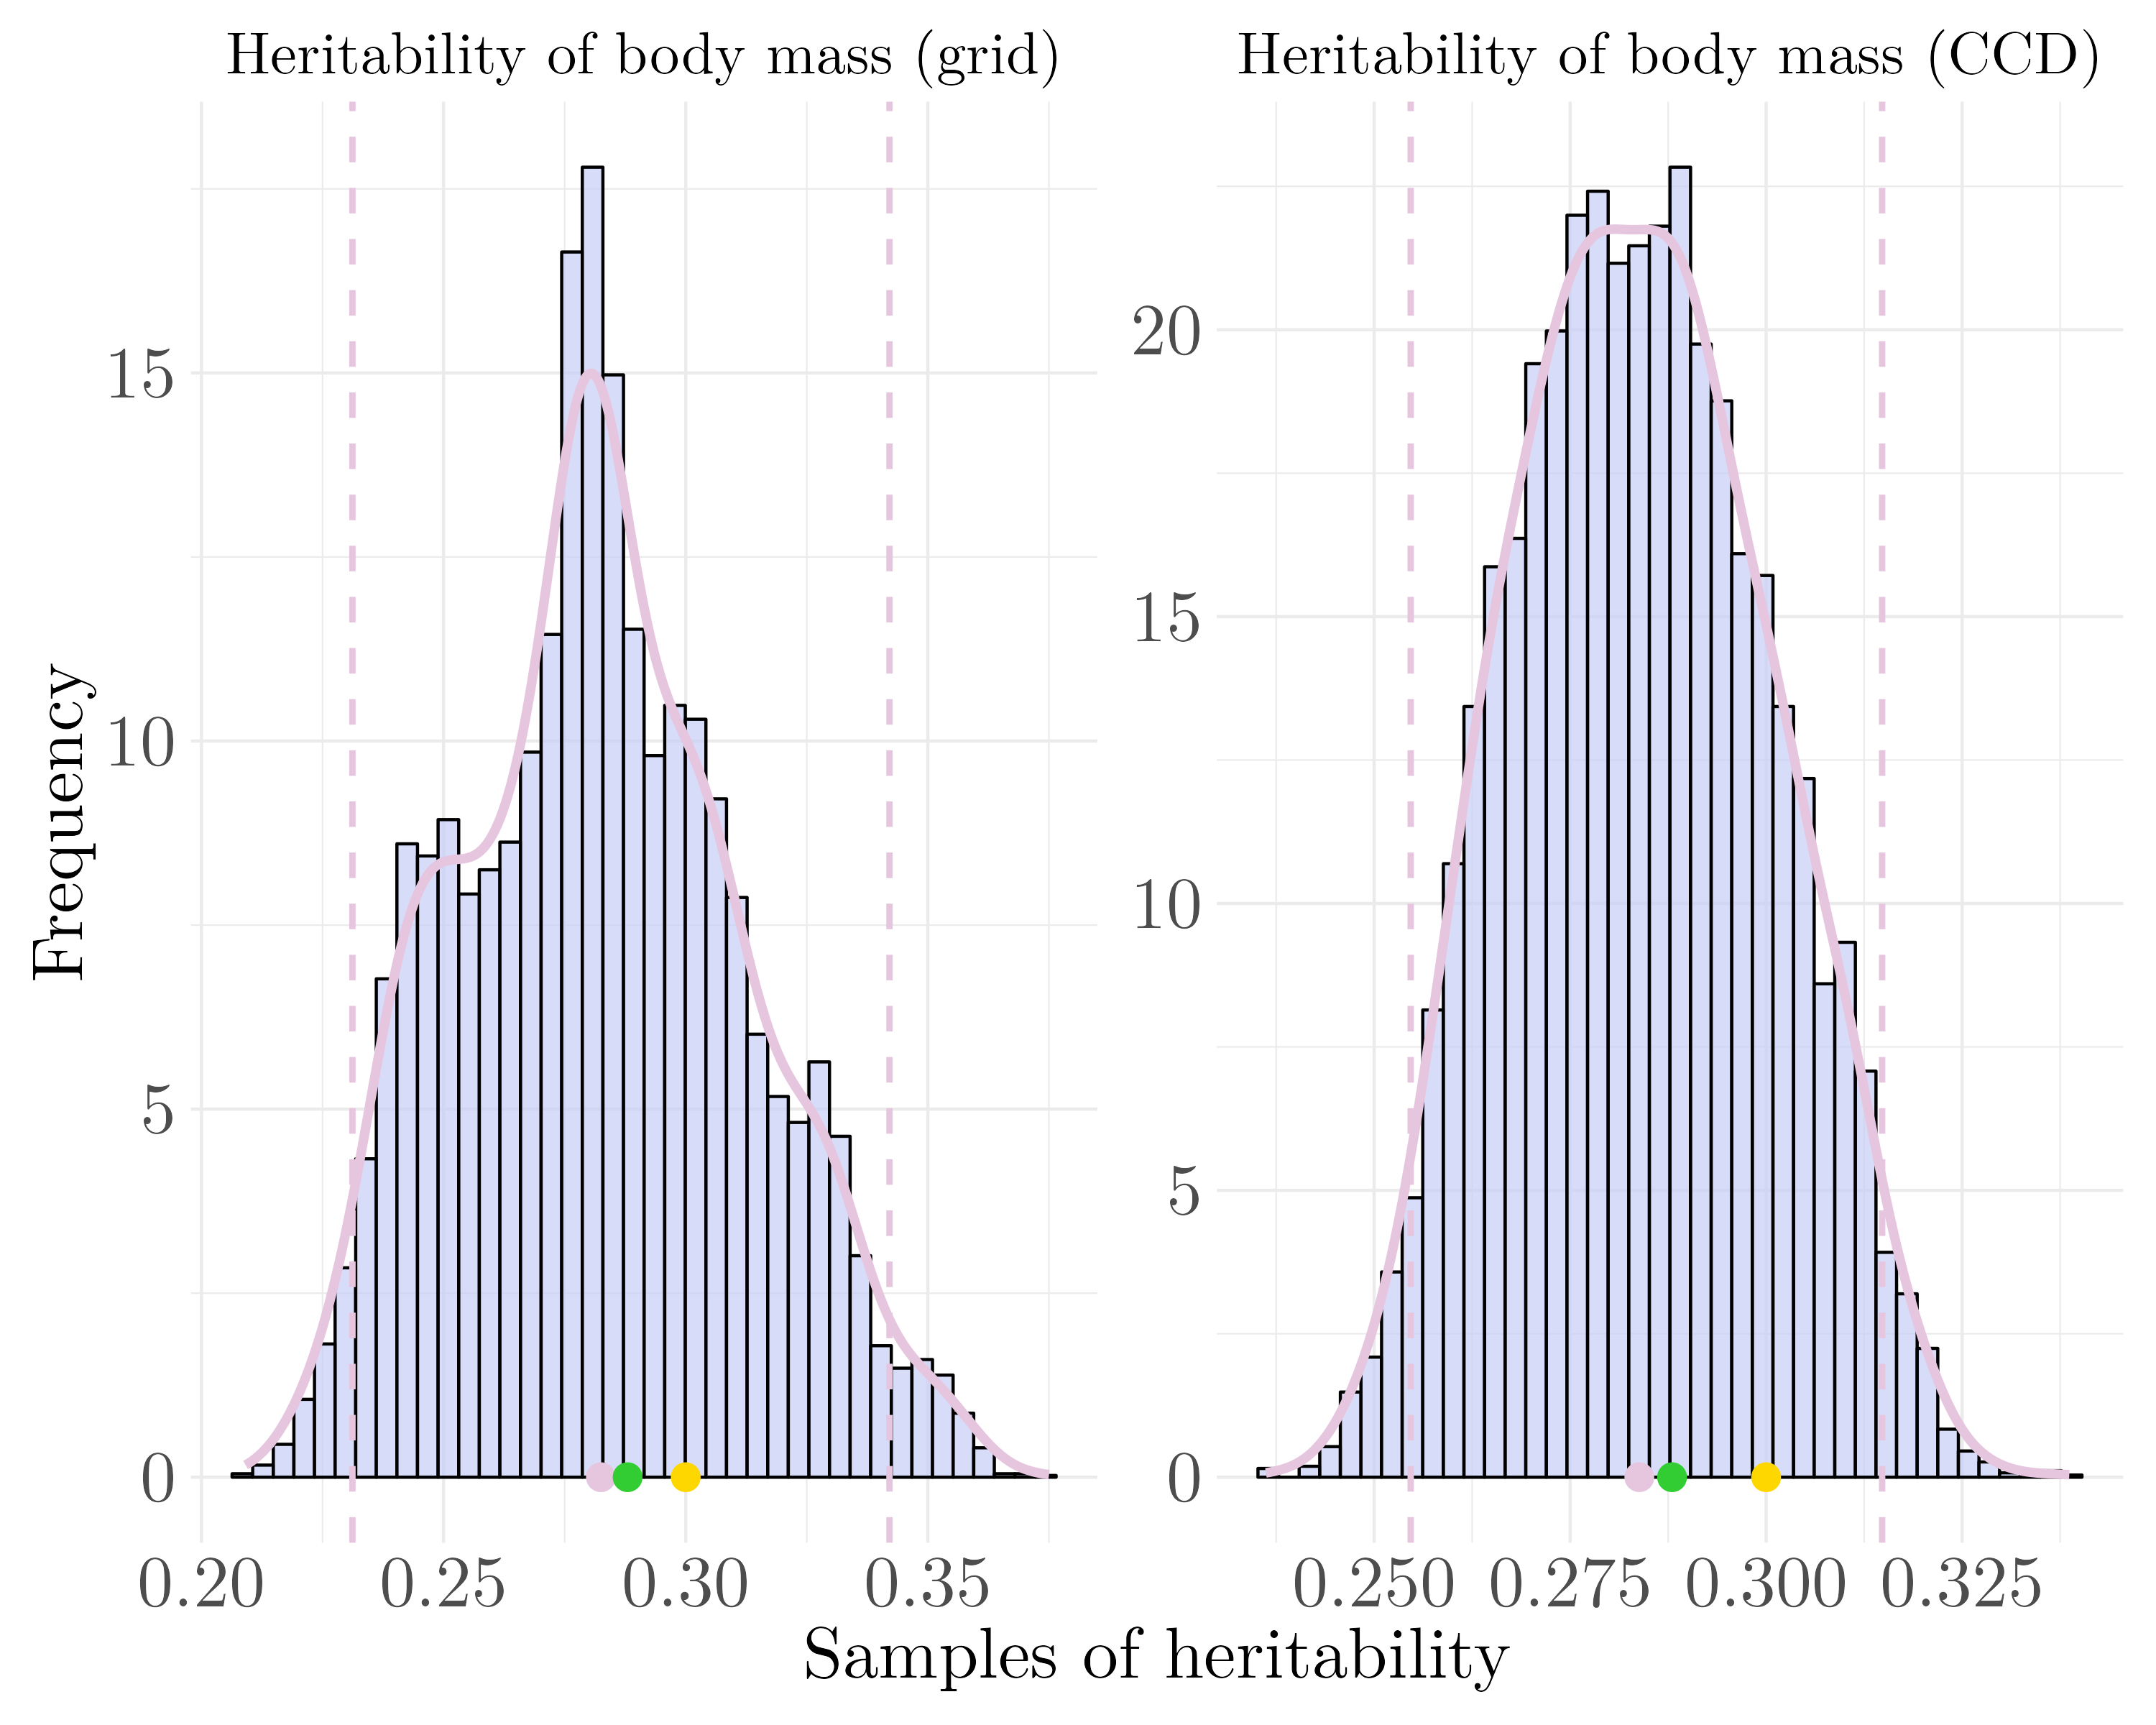
\includegraphics[width=0.7\linewidth]{Figures/House sparrow study/Heritability_mass_combined.png}
  \caption[Estimated heritability of body mass from grid and CCD strategy]{Histogram depicting the estimated heritability values of body mass by the BVI method for the grid integration strategy(left) and CCD integration strategy (right) for the house sparrow dataset. The mean of the samples is marked as a pink circle at the bottom of the histogram, with the lower and upper value for the $95\%$ percentile marked as dashed lines. The heritability estimate from \citet{Silva2017} and \citet{Muff2019Genetic} are marked as gold and green dots respectively at the bottom of the histogram.}
  \label{fig:heritability_mass_combined_grid_ccd}
\end{figure}

\begin{figure}[ht]
  \centering
  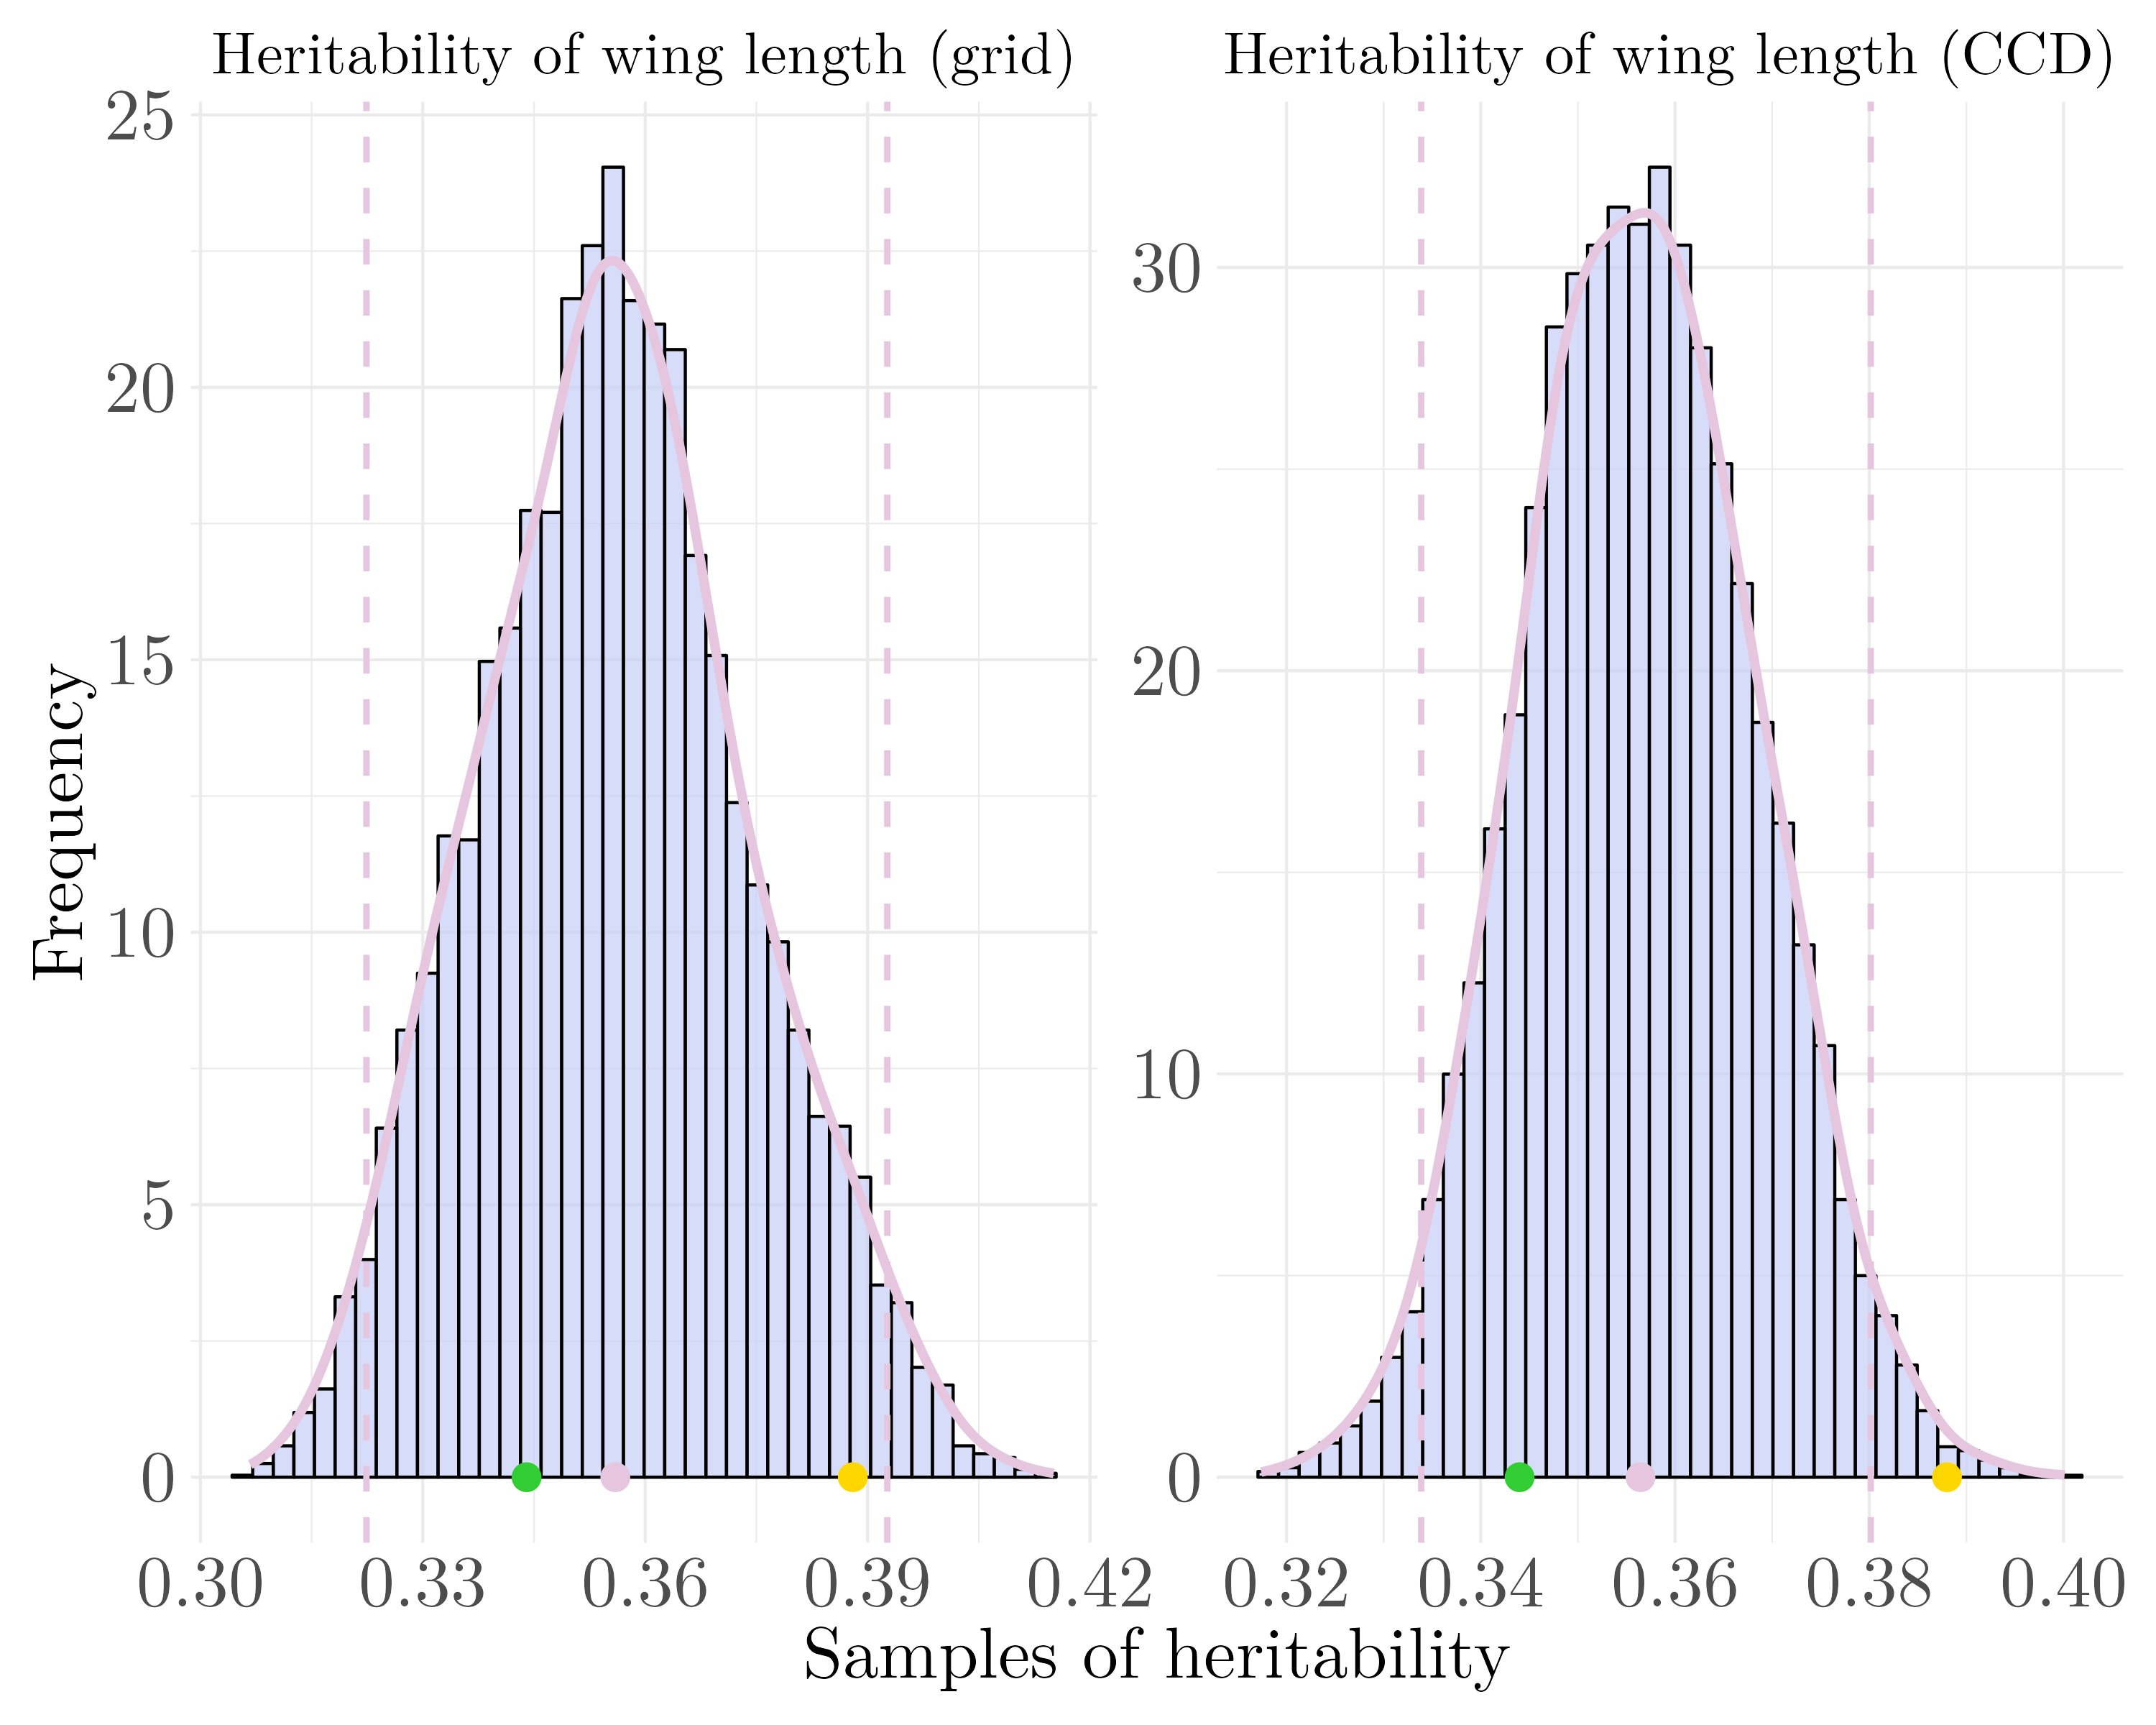
\includegraphics[width=0.7\linewidth]{Figures/House sparrow study/Heritability_wing_combined.png}
  \caption[Estimated heritability of wing length]{Histogram of heritability values for wing length of the house sparrows estimated by the BVI method for the grid integration strategy (left) and the CCD integration strategy (right). The mean of the samples is marked as a pink circle at the bottom of the histogram, and the lower and upper value for the $95\%$ percentile are featured as dashed lines. The heritability estimate from \citet{Silva2017} and \citet{Muff2019Genetic} are marked as gold and green dots respectively at the bottom of the histogram.}
  \label{fig:heritability_wing_combined_grid_ccd}
\end{figure}

\begin{figure}[H]
  \centering
  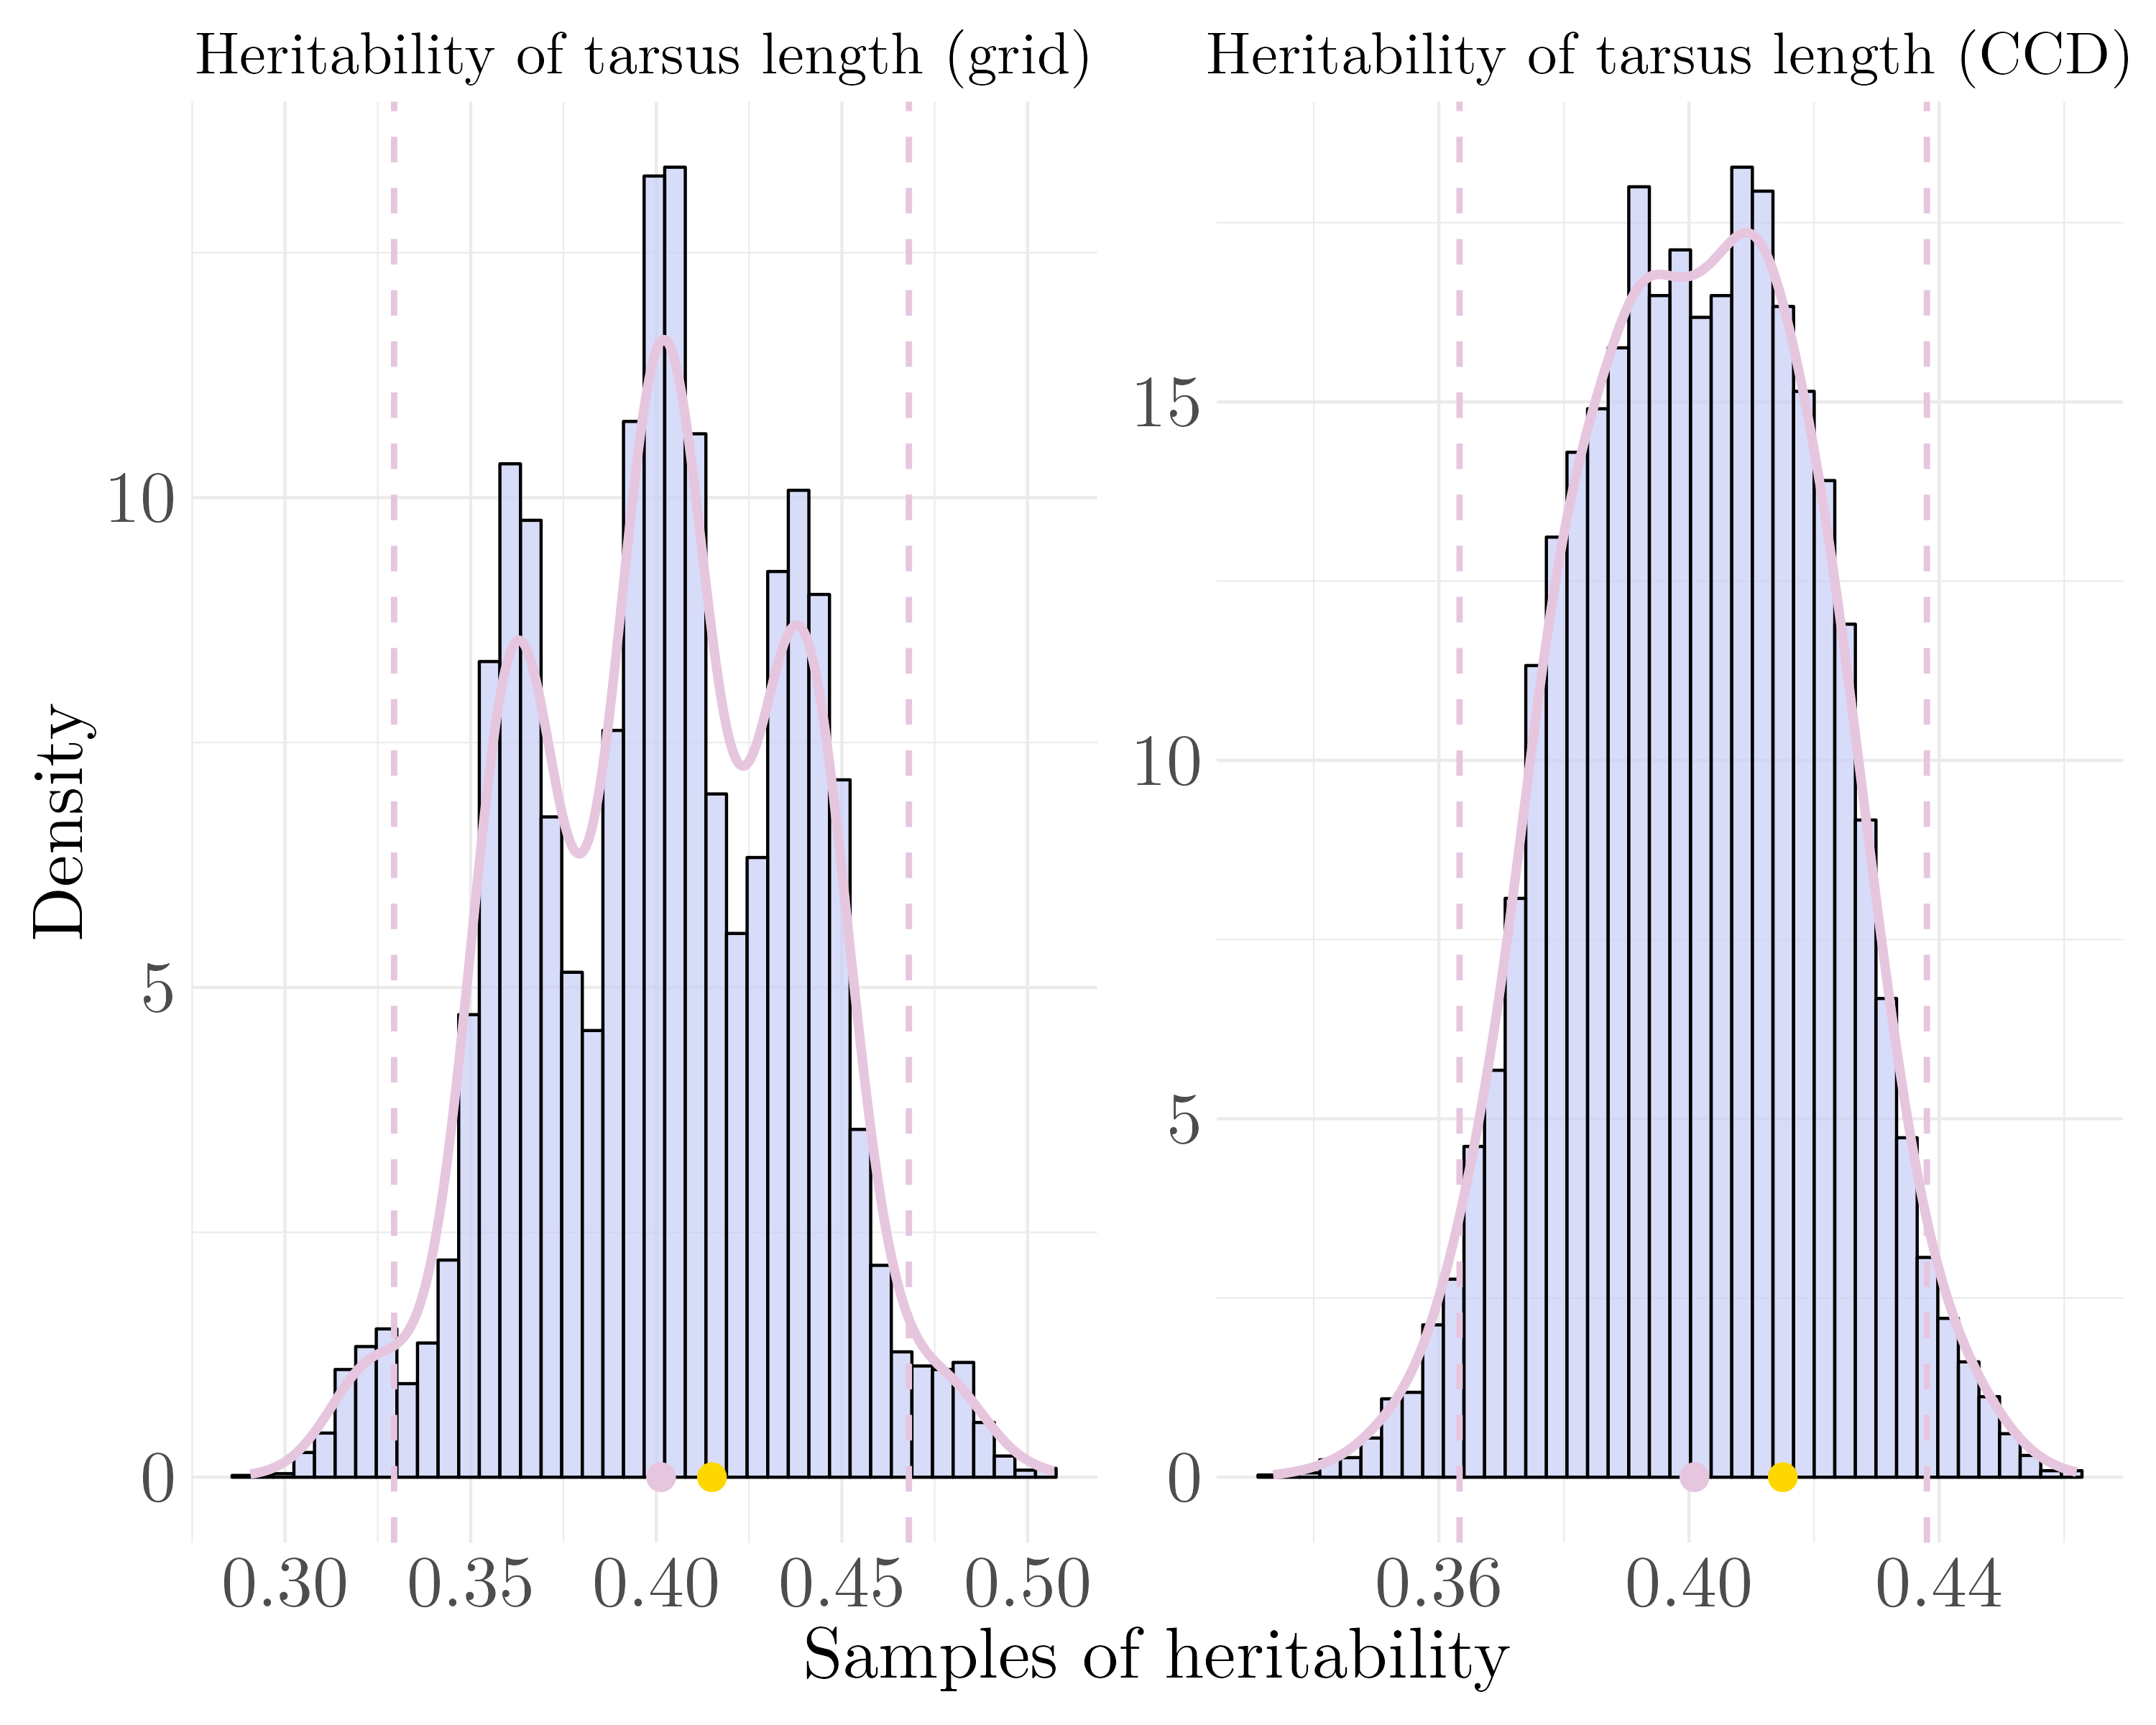
\includegraphics[width=0.7\linewidth]{Figures/House sparrow study/Heritability_tarsus_combined.png}
  \caption[Estimated heritability of tarsus length]{Histogram showing estimated heritability values for tarsus length of the house sparrows from the BVI method for the grid integration strategy (left) and the CCD integration strategy (right). The two dots at the bottom represent the mean of the samples (pink) and the estimate from \citep{Silva2017} (gold). The dashed lines represent the lower and upper value for the $95\%$ percentile.}
  \label{fig:heritability_tarsus_combined_grid_ccd}
\end{figure}
% \\
% \\
% The posterior distribution of relative importance of the fixed effects (\Cref{fig:mass_fixed_sparrows}) predominantly shows very small values. Both integration strategies yield very similar distributions. Notably, the covariates \textit{FGRM, age} and \textit{other} seem to have been allocated negligible importance, with the distributions of \textit{FGRM} and \textit{other} exhibiting a negative exponential decay pattern. Recall that importance calculations include squaring the coefficients, and so no negative importance can be allocated to a covariate. Therefore, the sharp decay from zero seems reasonable. The covariates \textit{month, sex} and \textit{outer} seem to have been allocated a small share of the importance, with \textit{month} and \textit{sex} showing signs of a normal distribution.
% \begin{figure}[H]%\ContinuedFloat
%   \centering
%   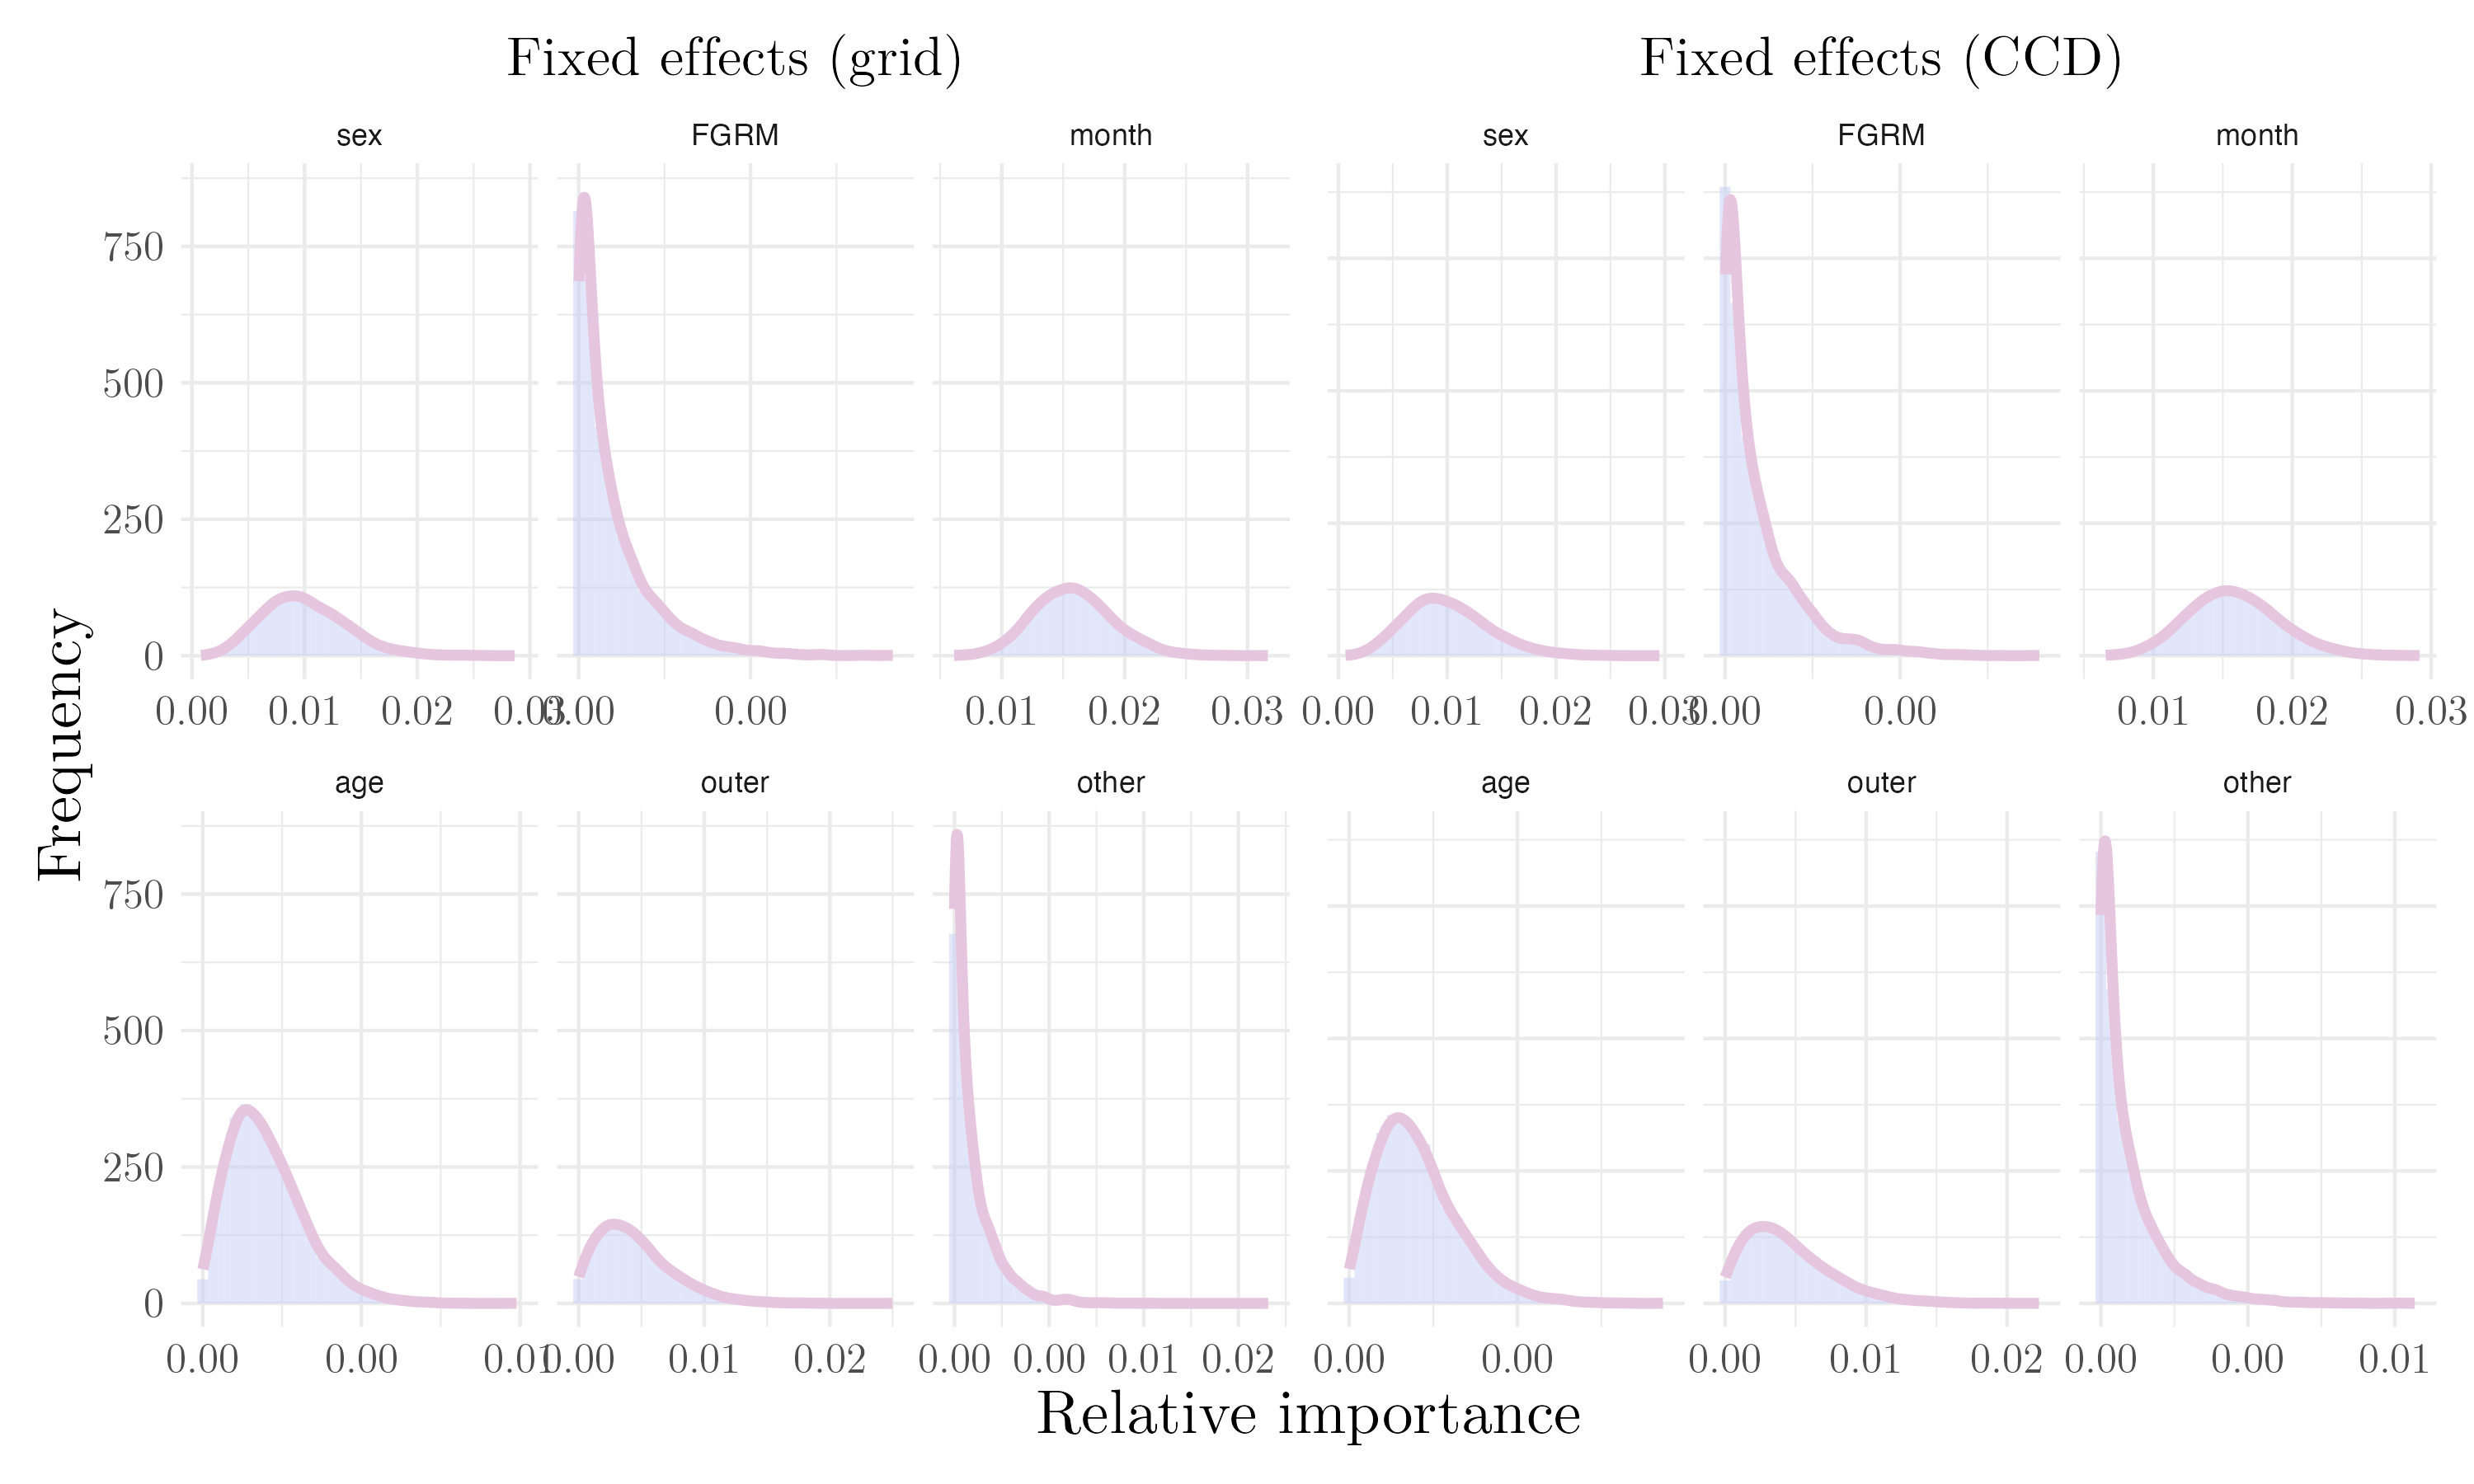
\includegraphics[width=1\linewidth]{Figures/House sparrow study/Mass_fixed.png}
%   \caption[Posterior relative importance distributions of all fixed effects in body mass model for house sparrow study]{Posterior relative importance distributions of all fixed effects in heritability of body mass model for house sparrow study. The grid integration is displayed on the left, and CCD on the right.}
%   \label{fig:mass_fixed_sparrows}
% \end{figure}
% When considering the posterior importance of the random effects (\Cref{fig:mass_random_sparrows}), it is evident that they have been allocated a much larger share of importance compared to the fixed effects. The Gaussian observations exhibit the largest influence, being allocated a share of over $0.5$ in both integration strategies. It seems that the CCD integration gives somewhat smoother distributions, but the mean values seem to be roughly similar. We notice a trimodal shape for the individual effect \textit{IDC} (overdispersion) with the grid integration strategy, similar to that observed for the heritability of tarsus length. The smallest importance of random effects is allocated to \textit{hatchyear}, and the estimates for covariate \textit{IDC2} corresponds to the heritability of body mass.
% \begin{figure}[H]%\ContinuedFloat
%   \centering
%   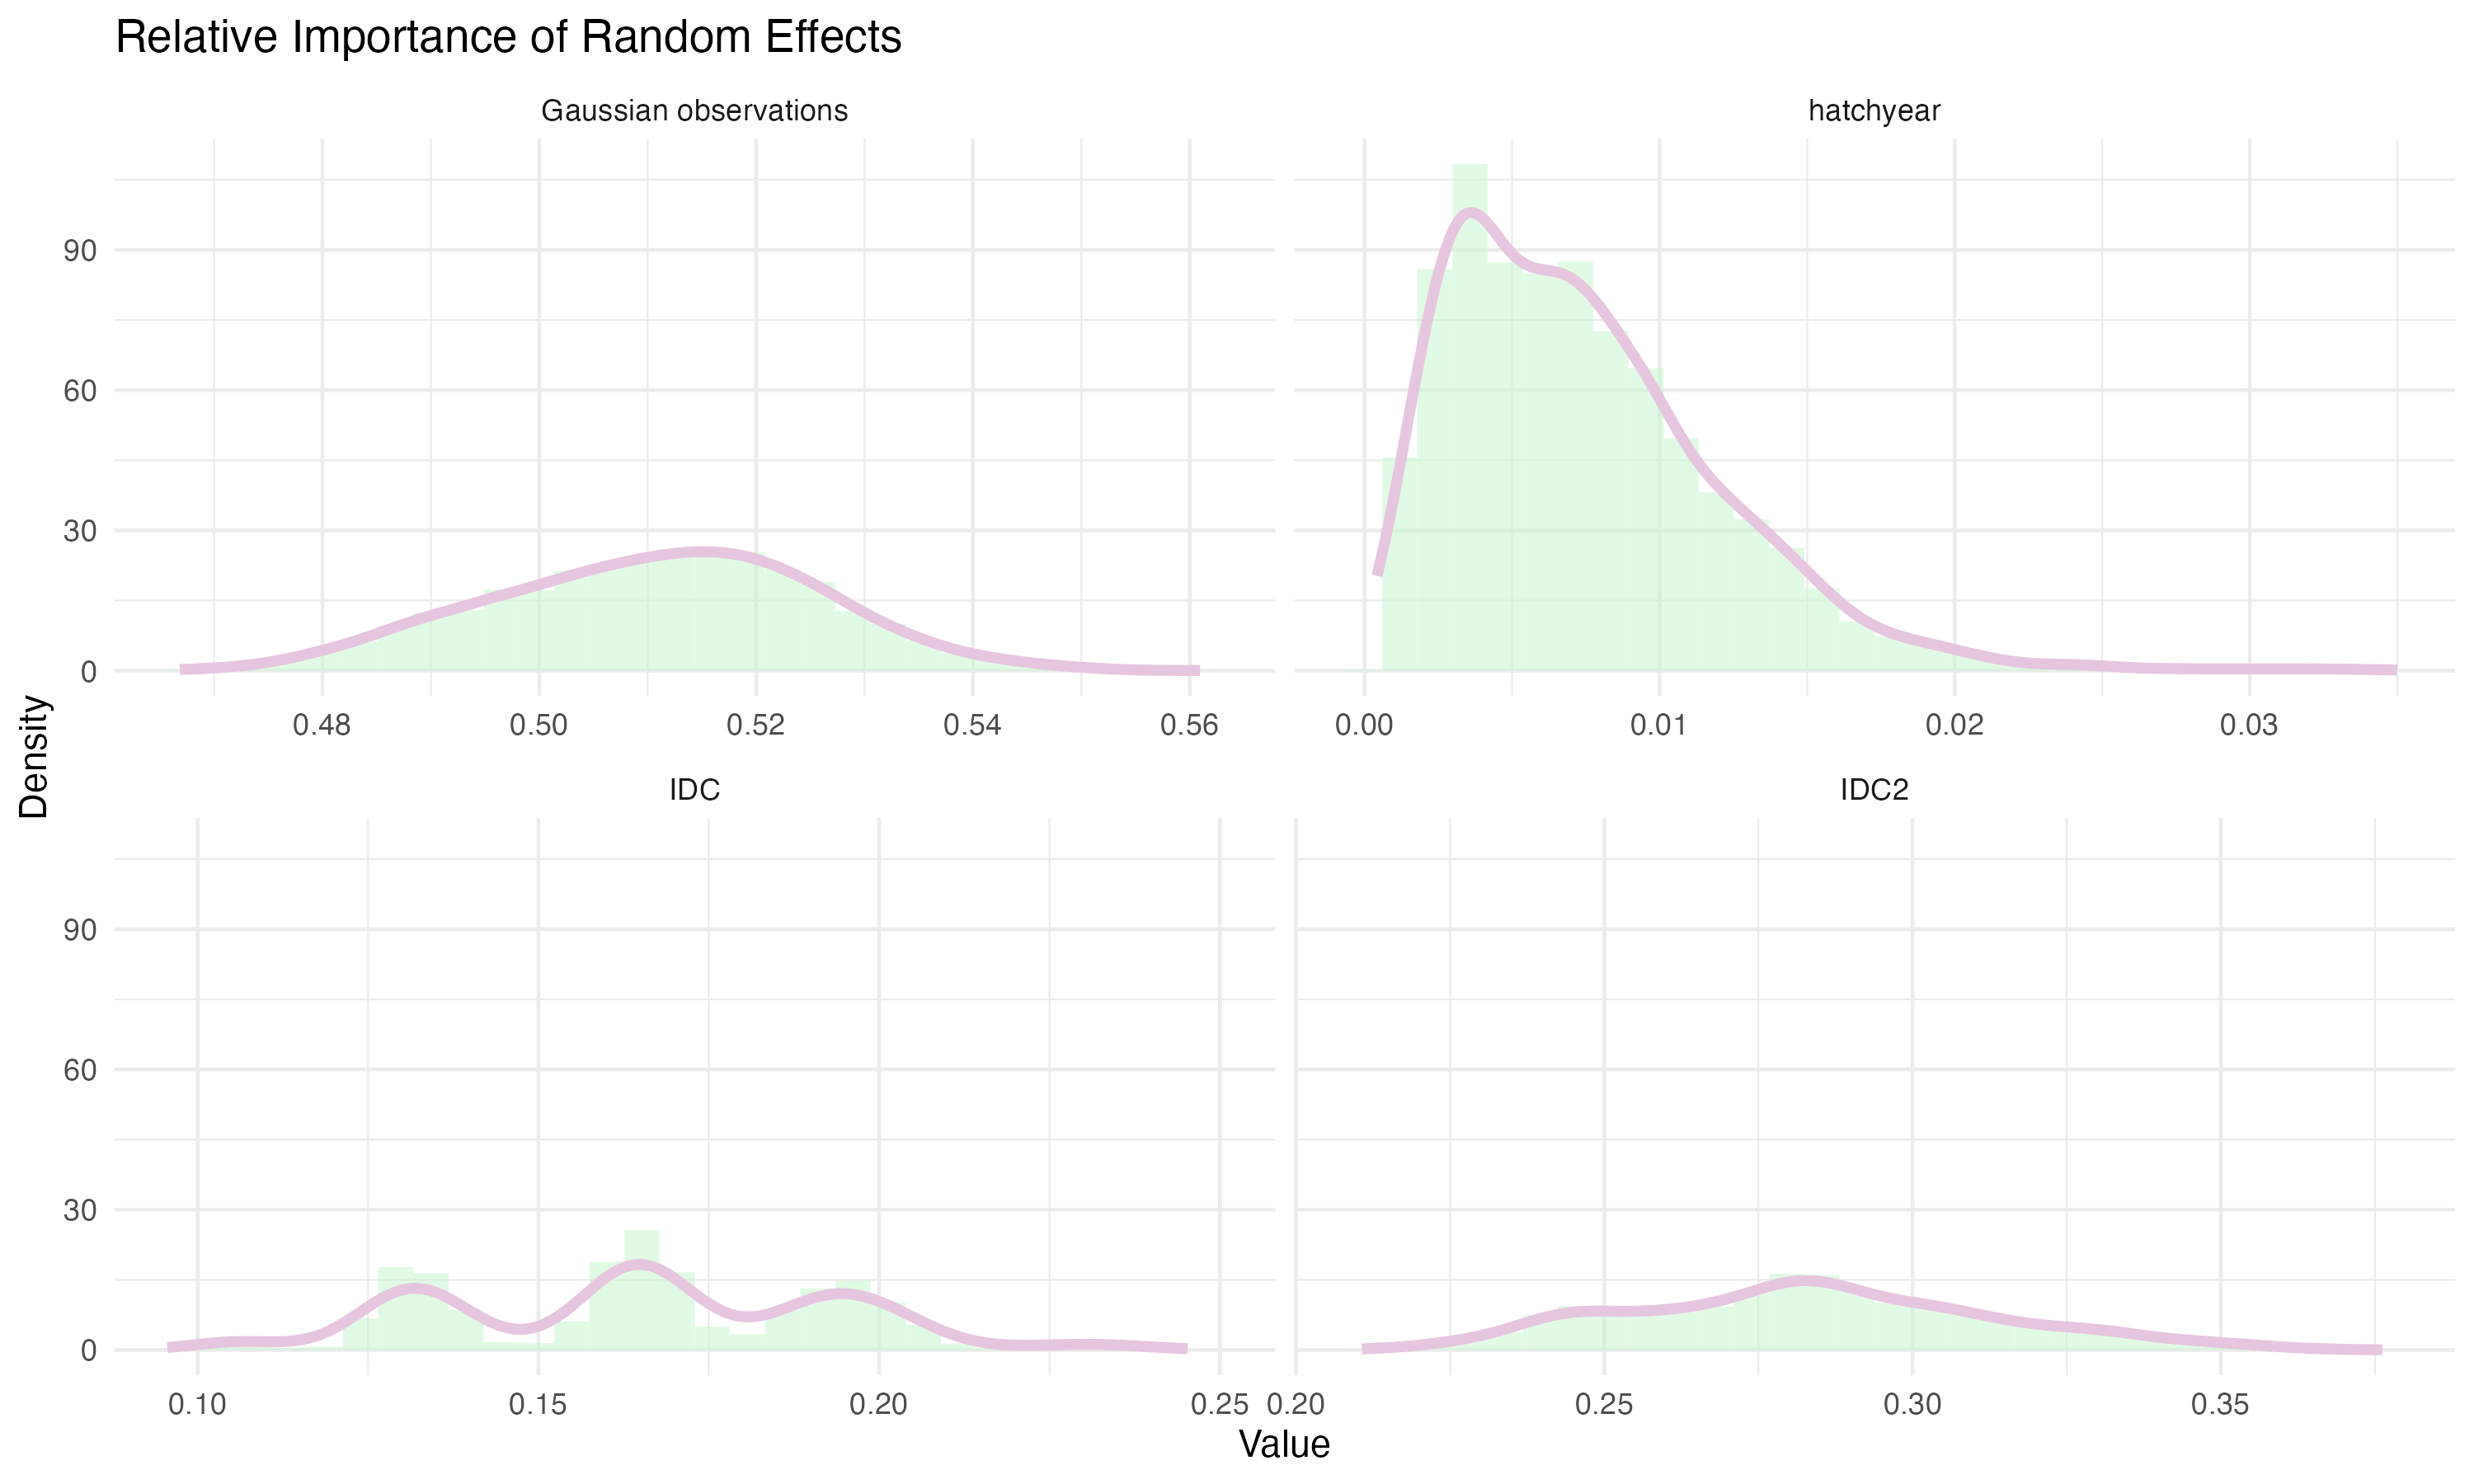
\includegraphics[width=1\linewidth]{Figures/House sparrow study/Mass_random.png}
%   \caption[Posterior relative importance distributions of all random effects in body mass model for house sparrow study]{Posterior relative importance distributions of all random effects in heritability of body mass model for house sparrow study. The grid integration is displayed on the left, and CCD on the right.}
%   \label{fig:mass_random_sparrows}
% \end{figure}
% As the marginal $R^2$ is the sum of the importance of fixed effects, the resulting estimates (\Cref{fig:mass_r2}) are expectedly very small. The conditional $R^2$ estimates are much larger, which is because this contains the importances of the random effects. All in all, the grid and CCD integrations yield similar results, with a slightly sharper peak for the conditional $R^2$ by the CCD integration. 
% \begin{figure}[H]%\ContinuedFloat
%   \centering
%   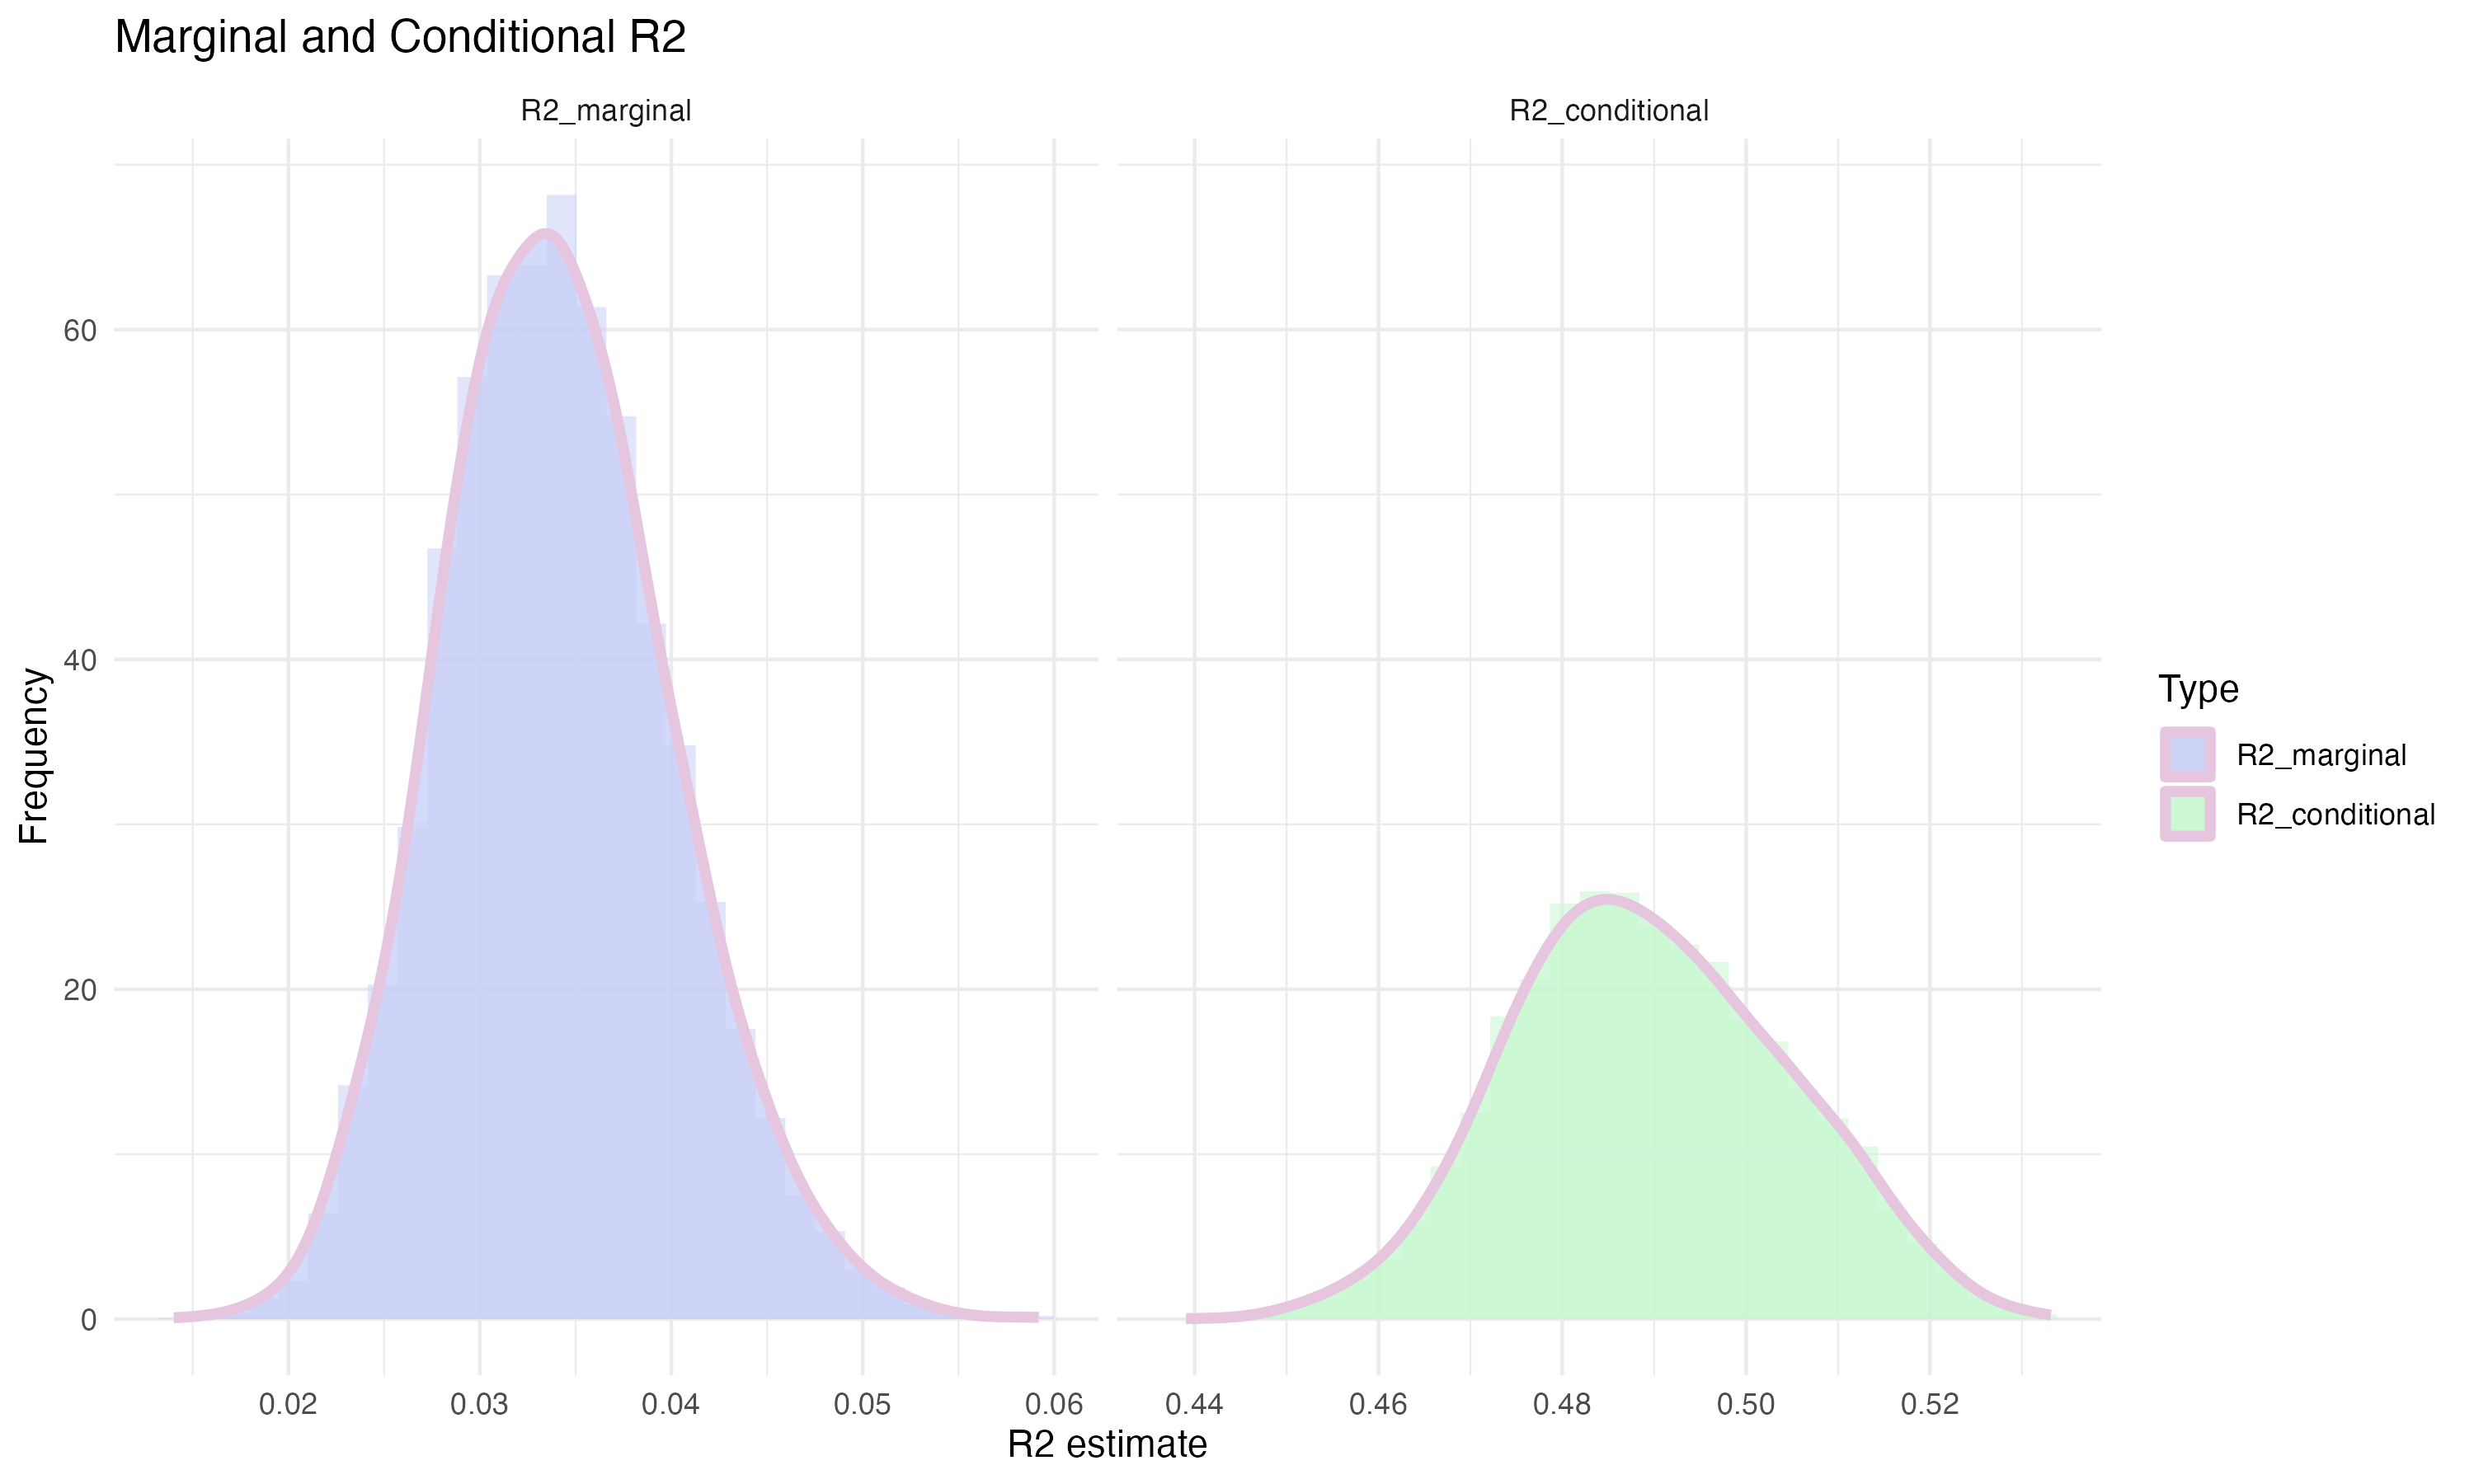
\includegraphics[width=1\linewidth]{Figures/House sparrow study/Mass_r2.png}
%   \caption[Posterior distributions of $R^2$ values in body mass model for house sparrow study]{Posterior distributions of $R^2$ values in heritability of body mass model for house sparrow study. The grid integration is displayed on the left, and CCD on the right.}
%   \label{fig:mass_r2}
% \end{figure}
% As for the fixed effects of the body mass model, the posterior importance of random effects for wing length (\Cref{fig:wing_fixed_sparrows}) are also generally very small except for the covariate \textit{sex}. The importance of covariate \textit{sex} seems to be normal around a value just below $0.35$, which is significantly larger than all other random effects. For wing length, \textit{FGRM} and \textit{other} are allocated a negligible importance, however they do not have the same negative exponential pattern as for body mass. Again, both integration strategies are in close agreement.
% \begin{figure}[H]%\ContinuedFloat
%   \centering
%   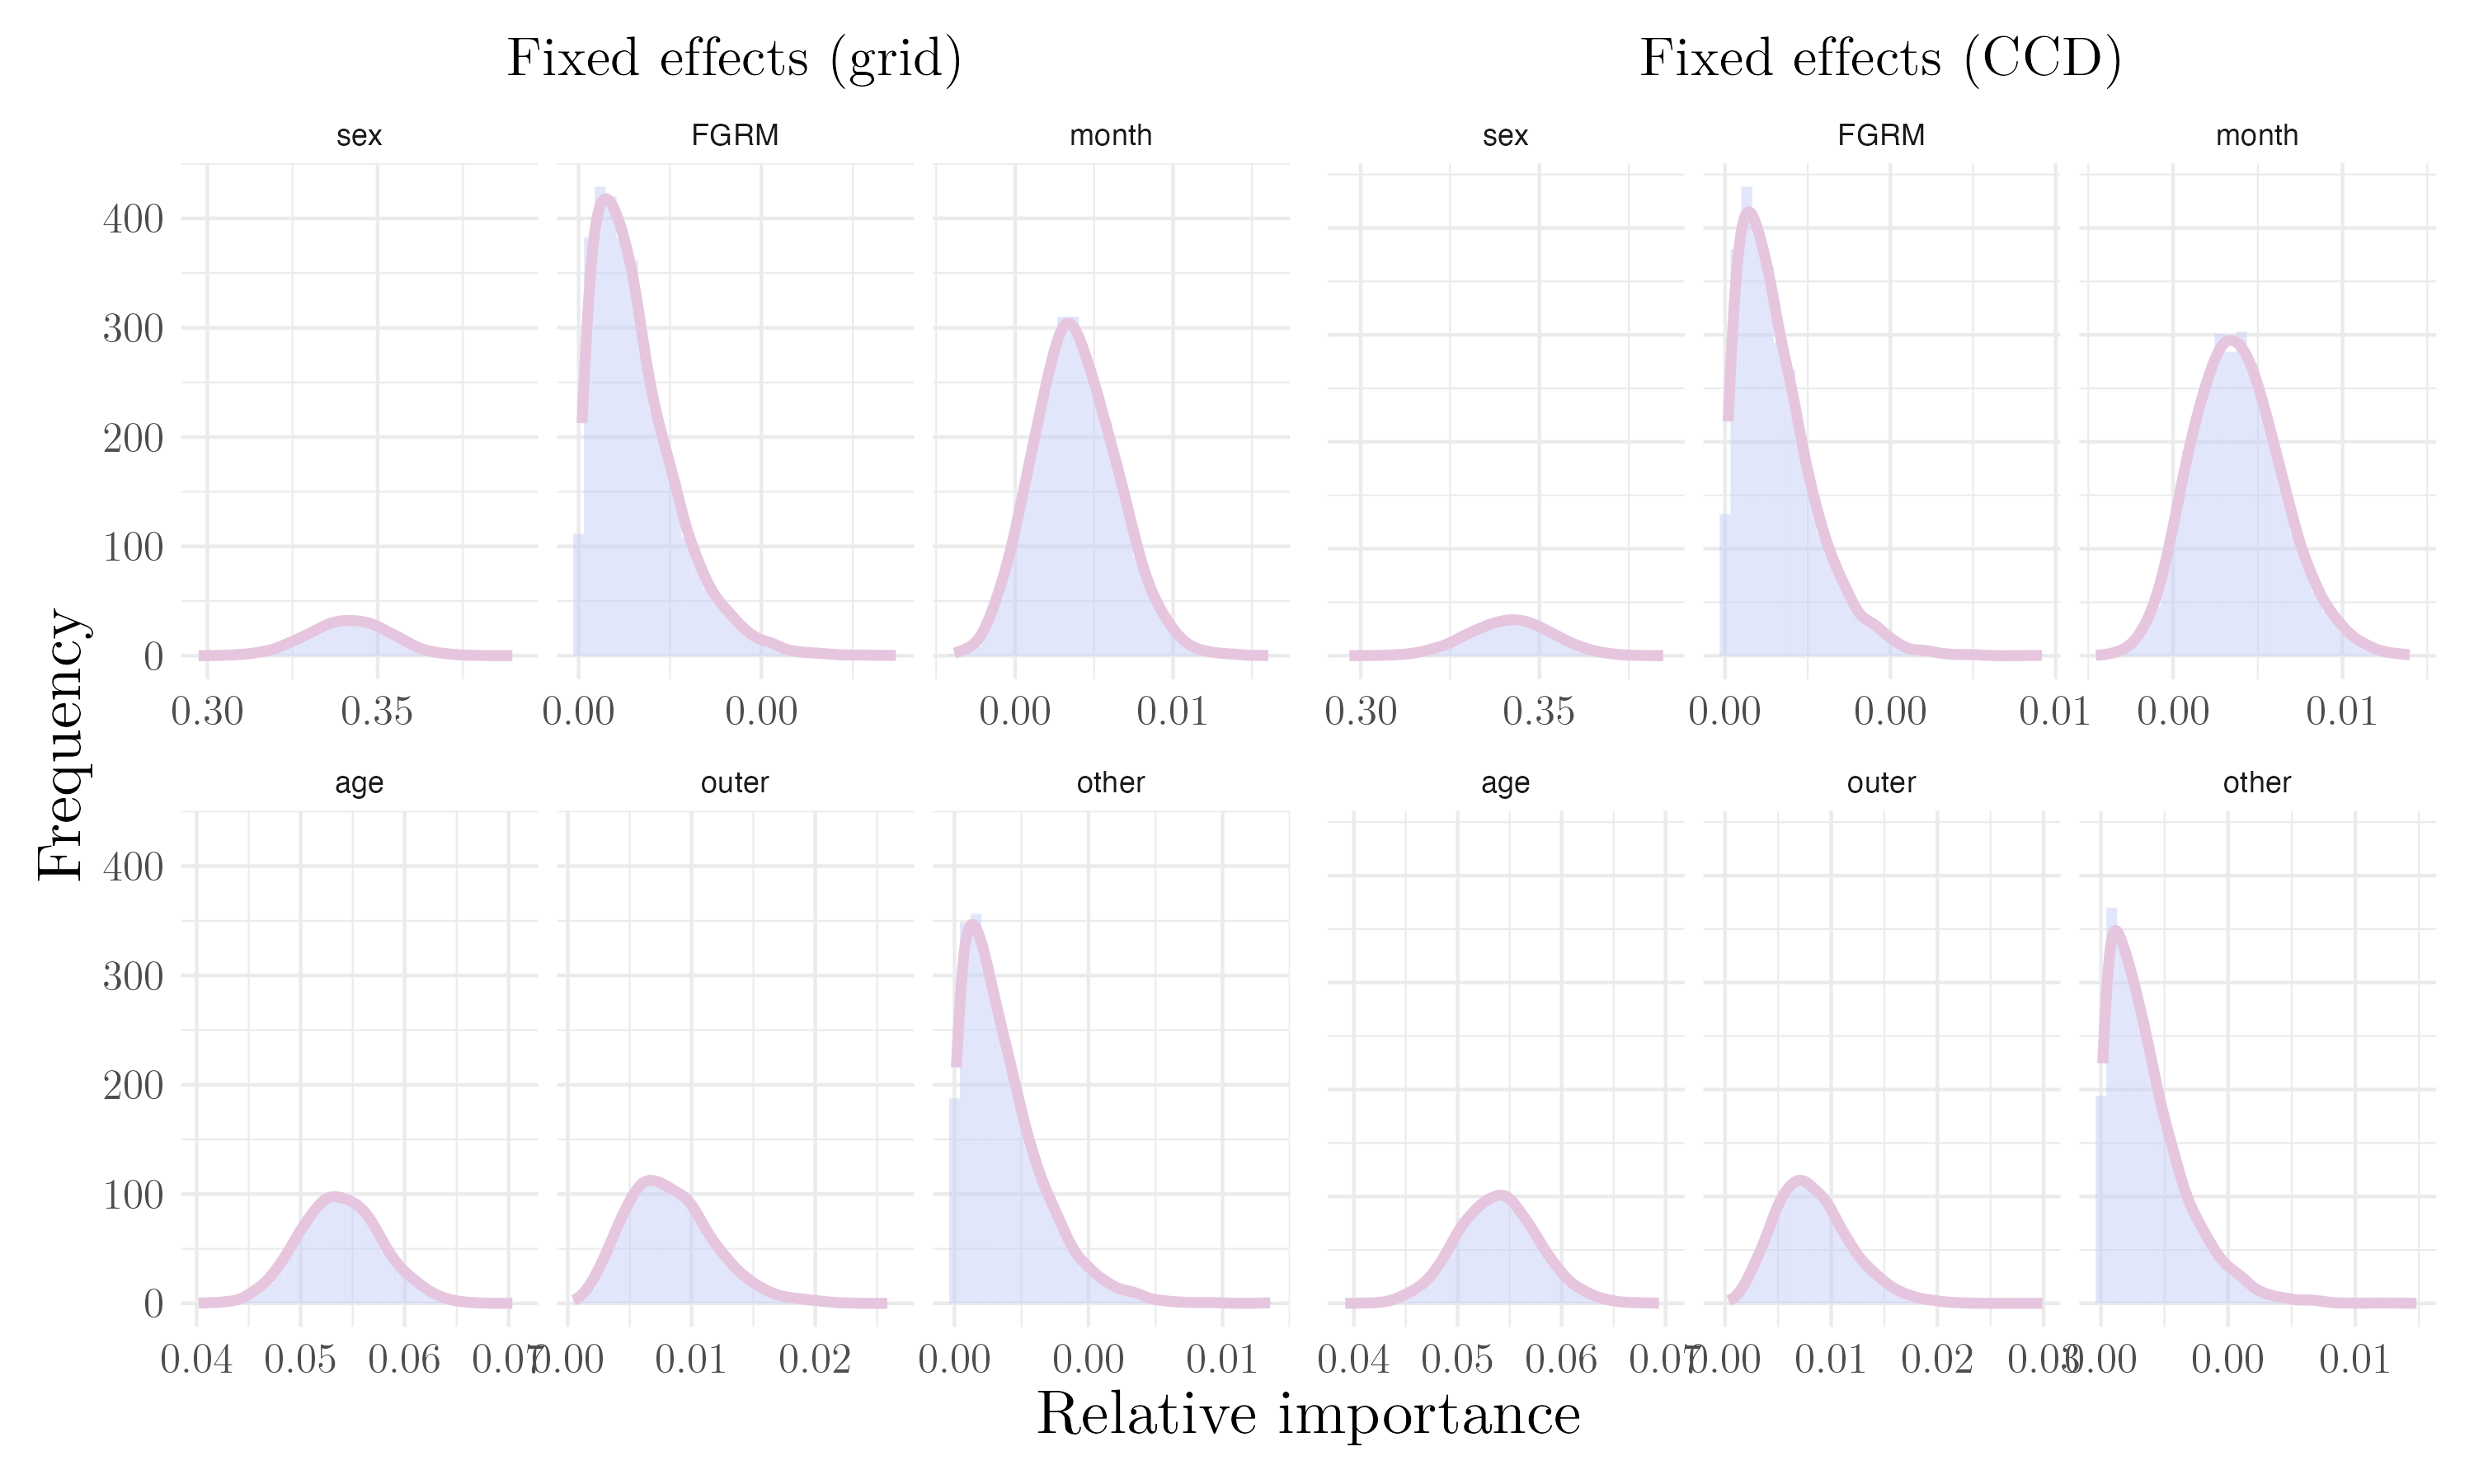
\includegraphics[width=1\linewidth]{Figures/House sparrow study/Wing_fixed.png}
%   \caption[Posterior relative importance distributions of all fixed effects in wing length model for house sparrow study]{Posterior relative importance distributions of all fixed effects in wing length model for house sparrow study. The grid integration is displayed on the left, and CCD on the right.}
%   \label{fig:wing_fixed_sparrows}
% \end{figure}
% For posterior importance of the random effects in the model for wing length (\Cref{fig:wing_random_sparrows}), the Gaussian observations are given an importance distributed around $0.175$. This is smaller than for body mass, and the \textit{IDC} covariate is also attributed significantly less importance when modelling wing length. The importance of \textit{hatchyear} is again quite small, and the importance of \textit{IDC2} (heritability) is now distributed around $0.36$. Once more, we observe the trimodal pattern for the importance of \textit{IDC} with the grid strategy. The CCD integrations also shows signs of a trimodal pattern for \textit{IDC}, but the peaks are less pronounced. 
% \begin{figure}[H]%\ContinuedFloat
%   \centering
%   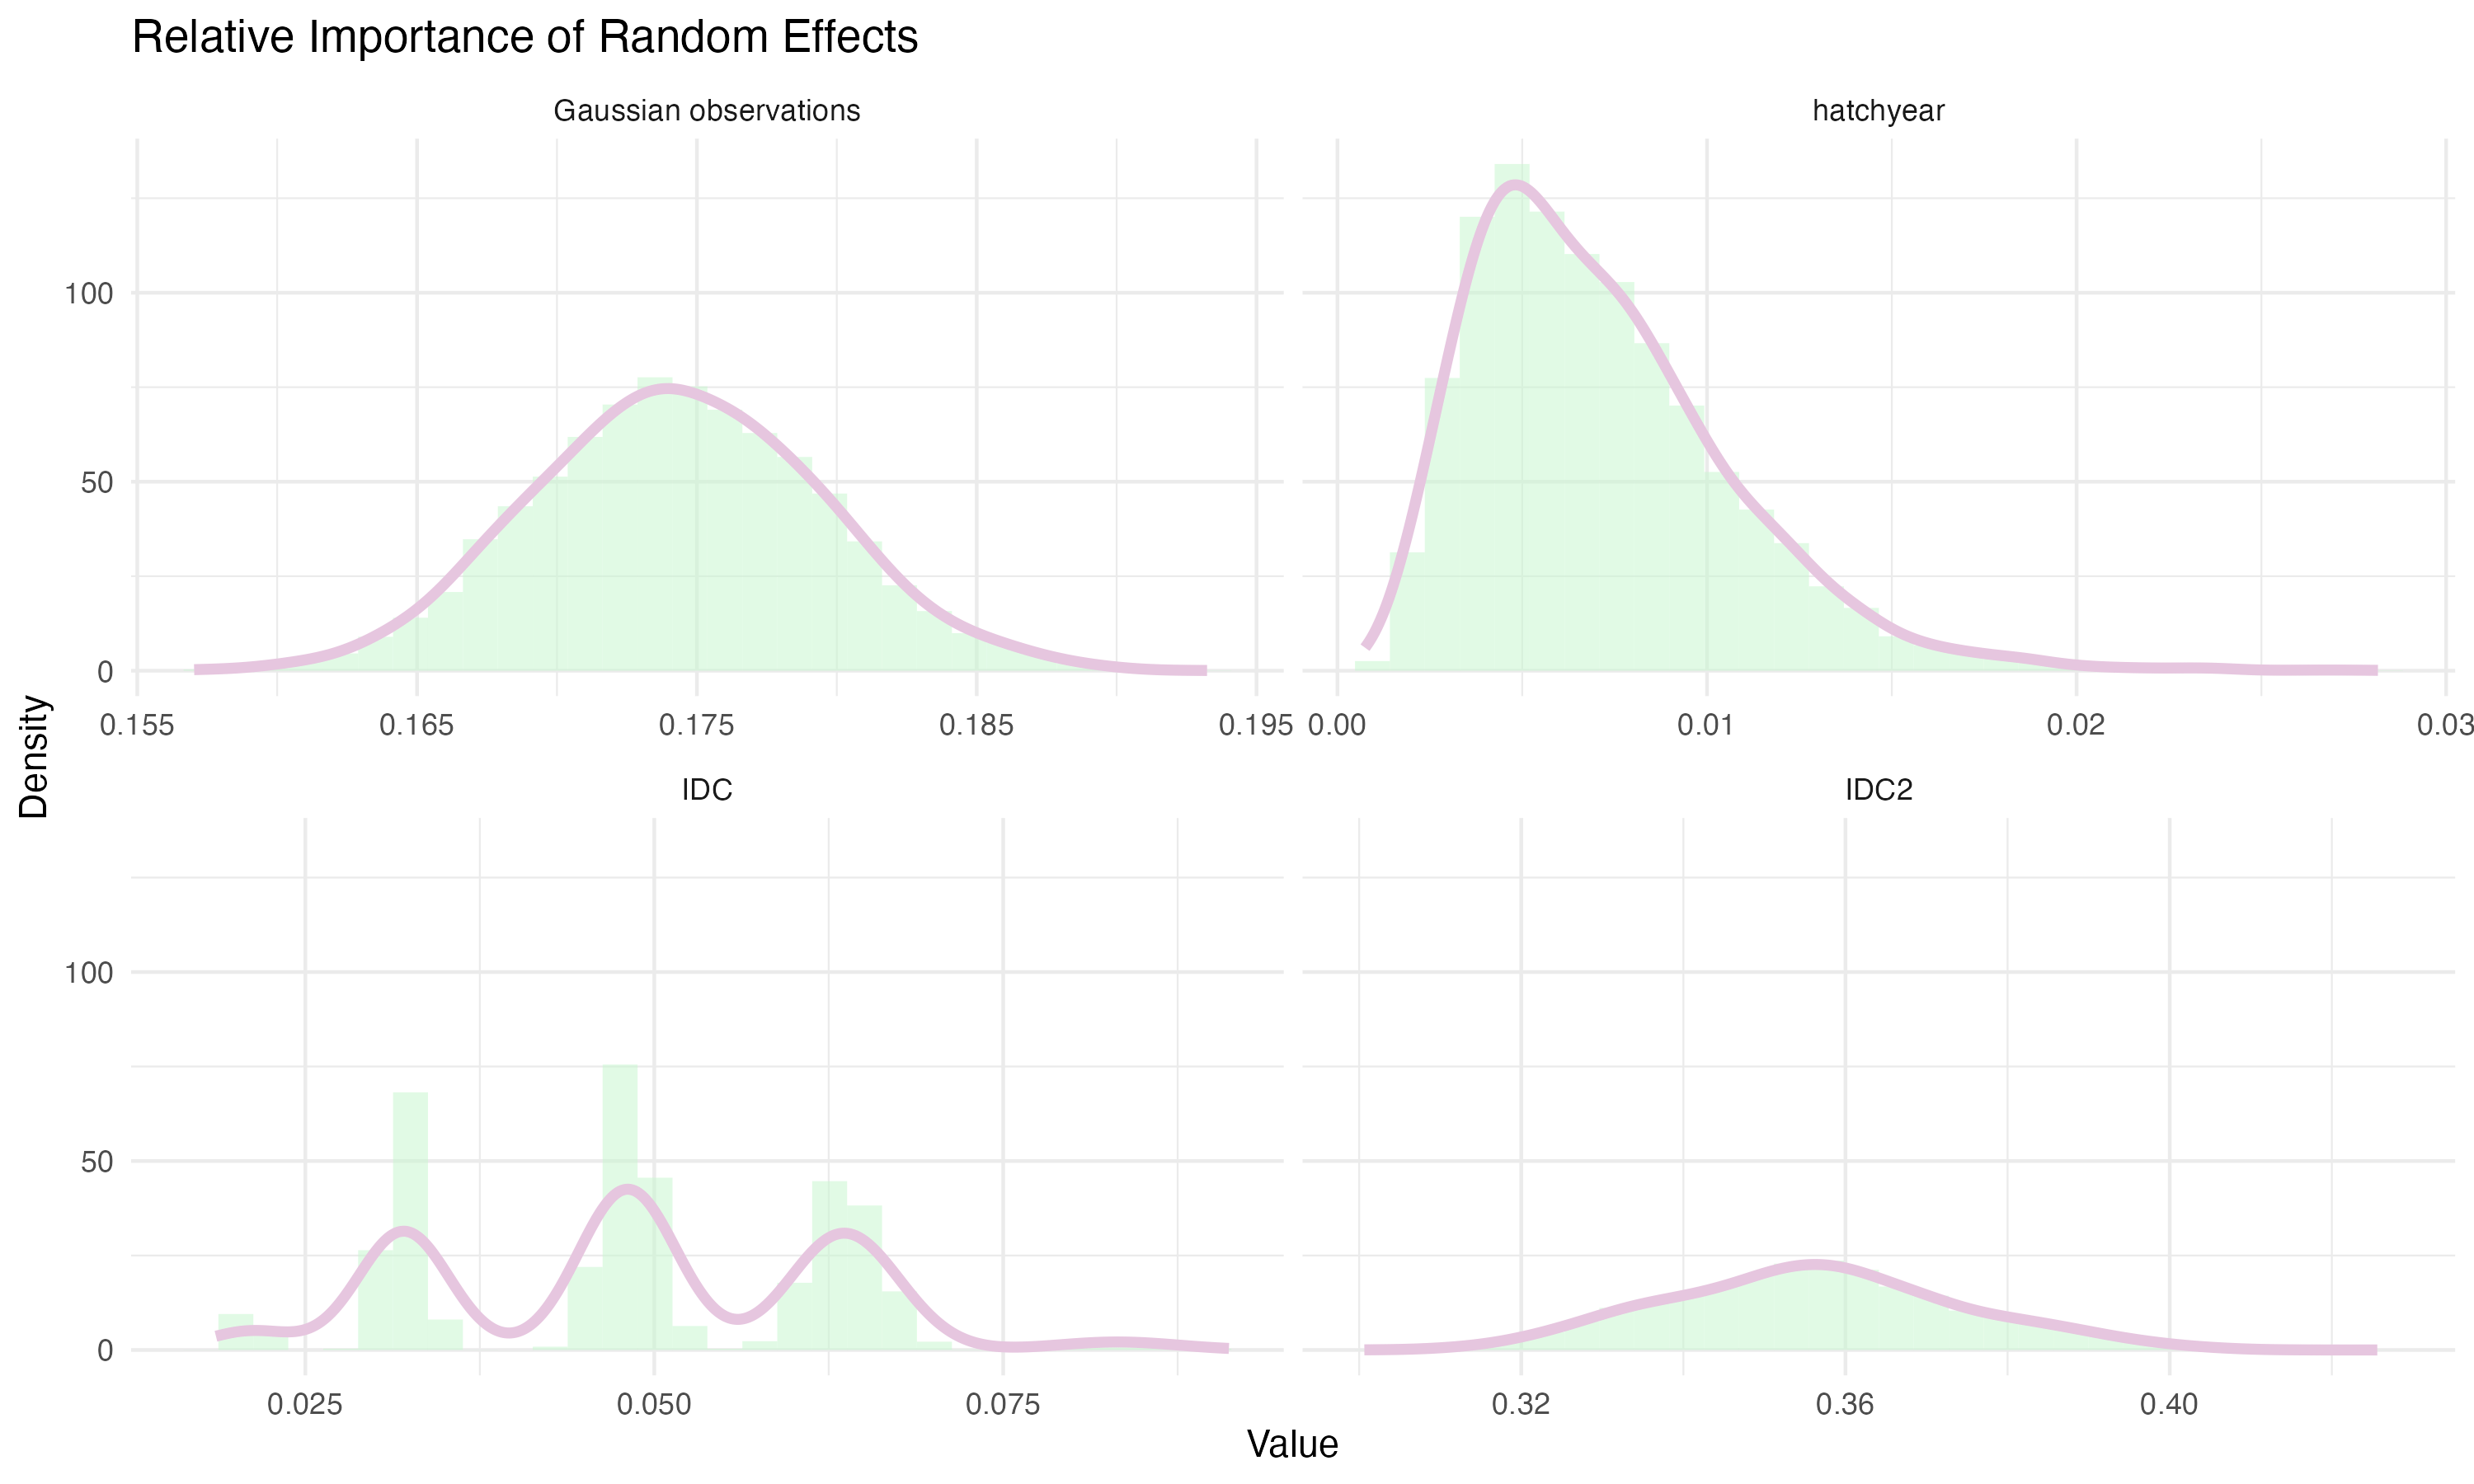
\includegraphics[width=1\linewidth]{Figures/House sparrow study/Wing_random.png}
%   \caption[Posterior relative importance distributions of all random effects in wing length model for house sparrow study]{Posterior relative importance distributions of all random effects in heritability of wing length model for house sparrow study. The grid integration is displayed on the left, and CCD on the right.}
%   \label{fig:wing_random_sparrows}
% \end{figure}
% Both the marginal and conditional $R^2$ of the wing length model (\Cref{fig:wing_r2}) are relatively large, which is a consequence of \textit{sex} being allocated a larger importance and the smaller importance allocated to the Gaussian observations. In this case, the peaks of the $R^2$ values with CCD integration are slightly sharper than for the grid integration, but the overall patterns are consistent across both methods.
% \begin{figure}[H]%\ContinuedFloat
%   \centering
%   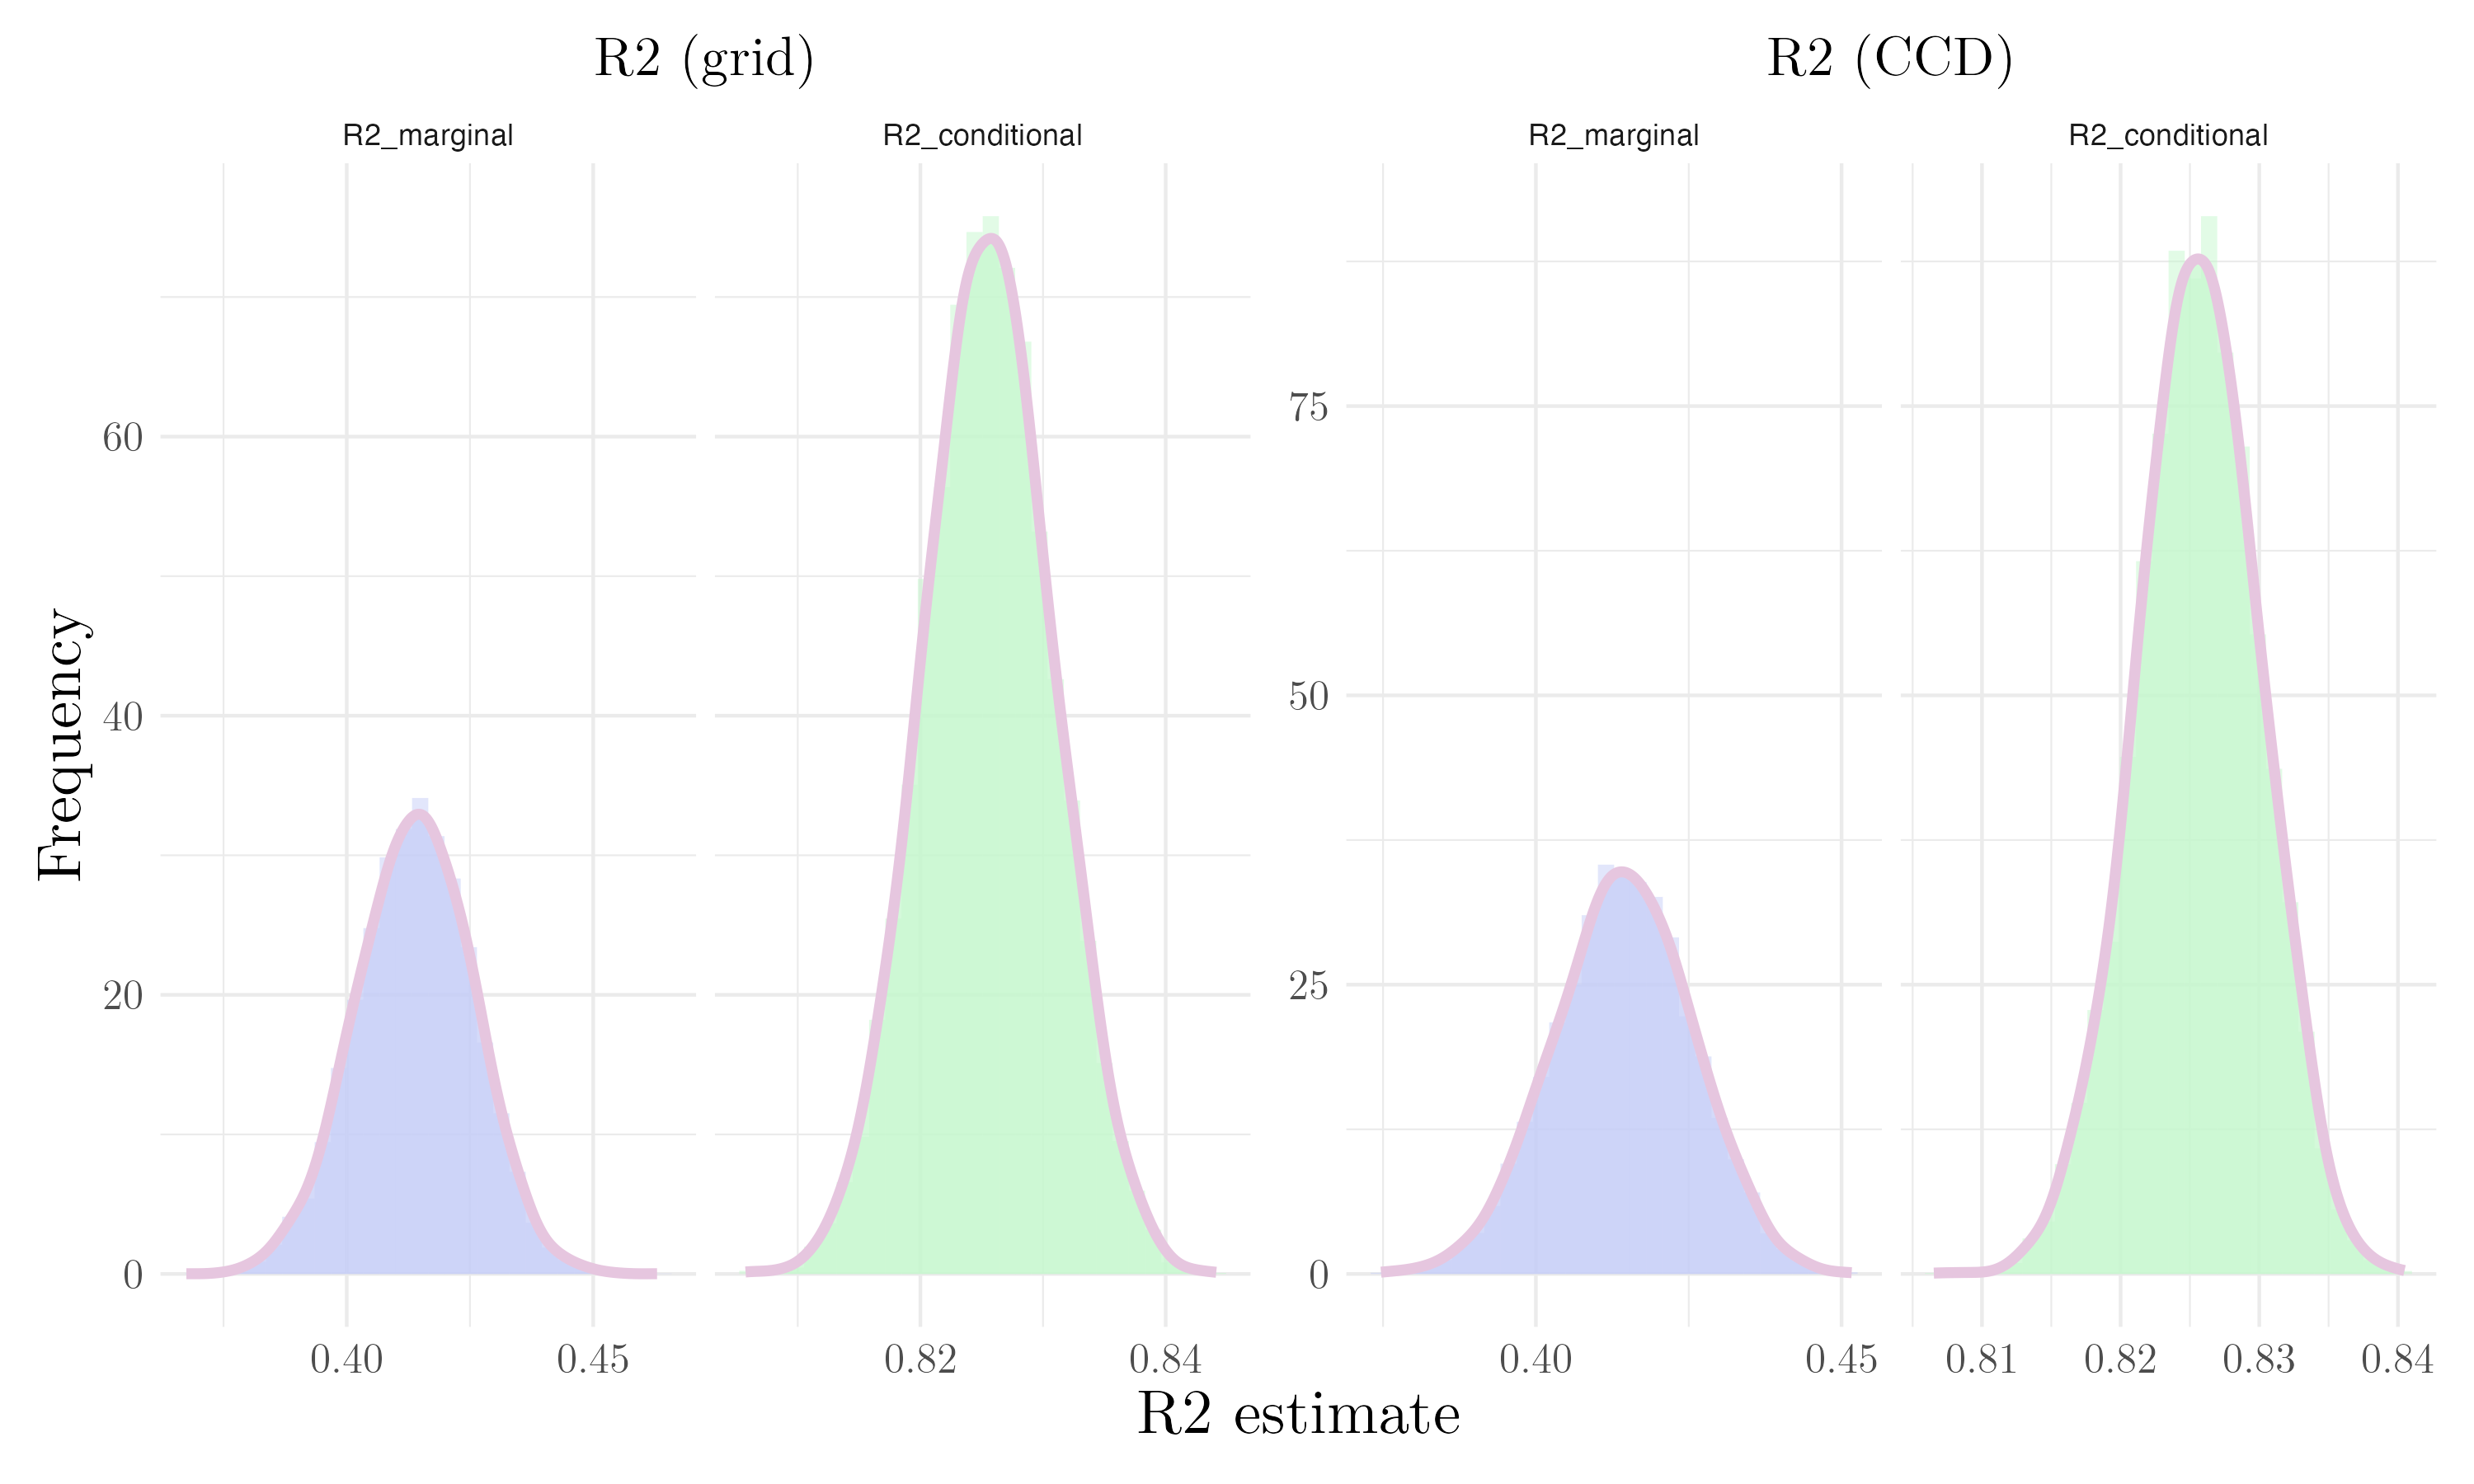
\includegraphics[width=1\linewidth]{Figures/House sparrow study/Wing_r2.png}
%   \caption[Posterior distributions of $R^2$ values in wing length model for house sparrow study]{Posterior distributions of $R^2$ values in heritability of wing length model for house sparrow study. The grid integration is displayed on the left, and CCD on the right.}
%   \label{fig:wing_r2}
% \end{figure}
% The posterior importance of fixed effects of the tarsus length model (\Cref{fig:tarsus_fixed_sparrows}) are challenging to interpret due to their minimal values. The covariate \textit{age} has a sharp decay right after zero with an extremely high frequency. Individually examining each importance distribution reveals that \textit{outer} and \textit{other} exhibit a negative exponential pattern, whereas \textit{month} follows a normal distribution.. Both \textit{sex} and \textit{FGRM} are very small and have a skewed normal distribution. It seems the integration strategies agree, and overall the fixed effects are given a very small importance.
% \begin{figure}[H]%\ContinuedFloat
%   \centering
%   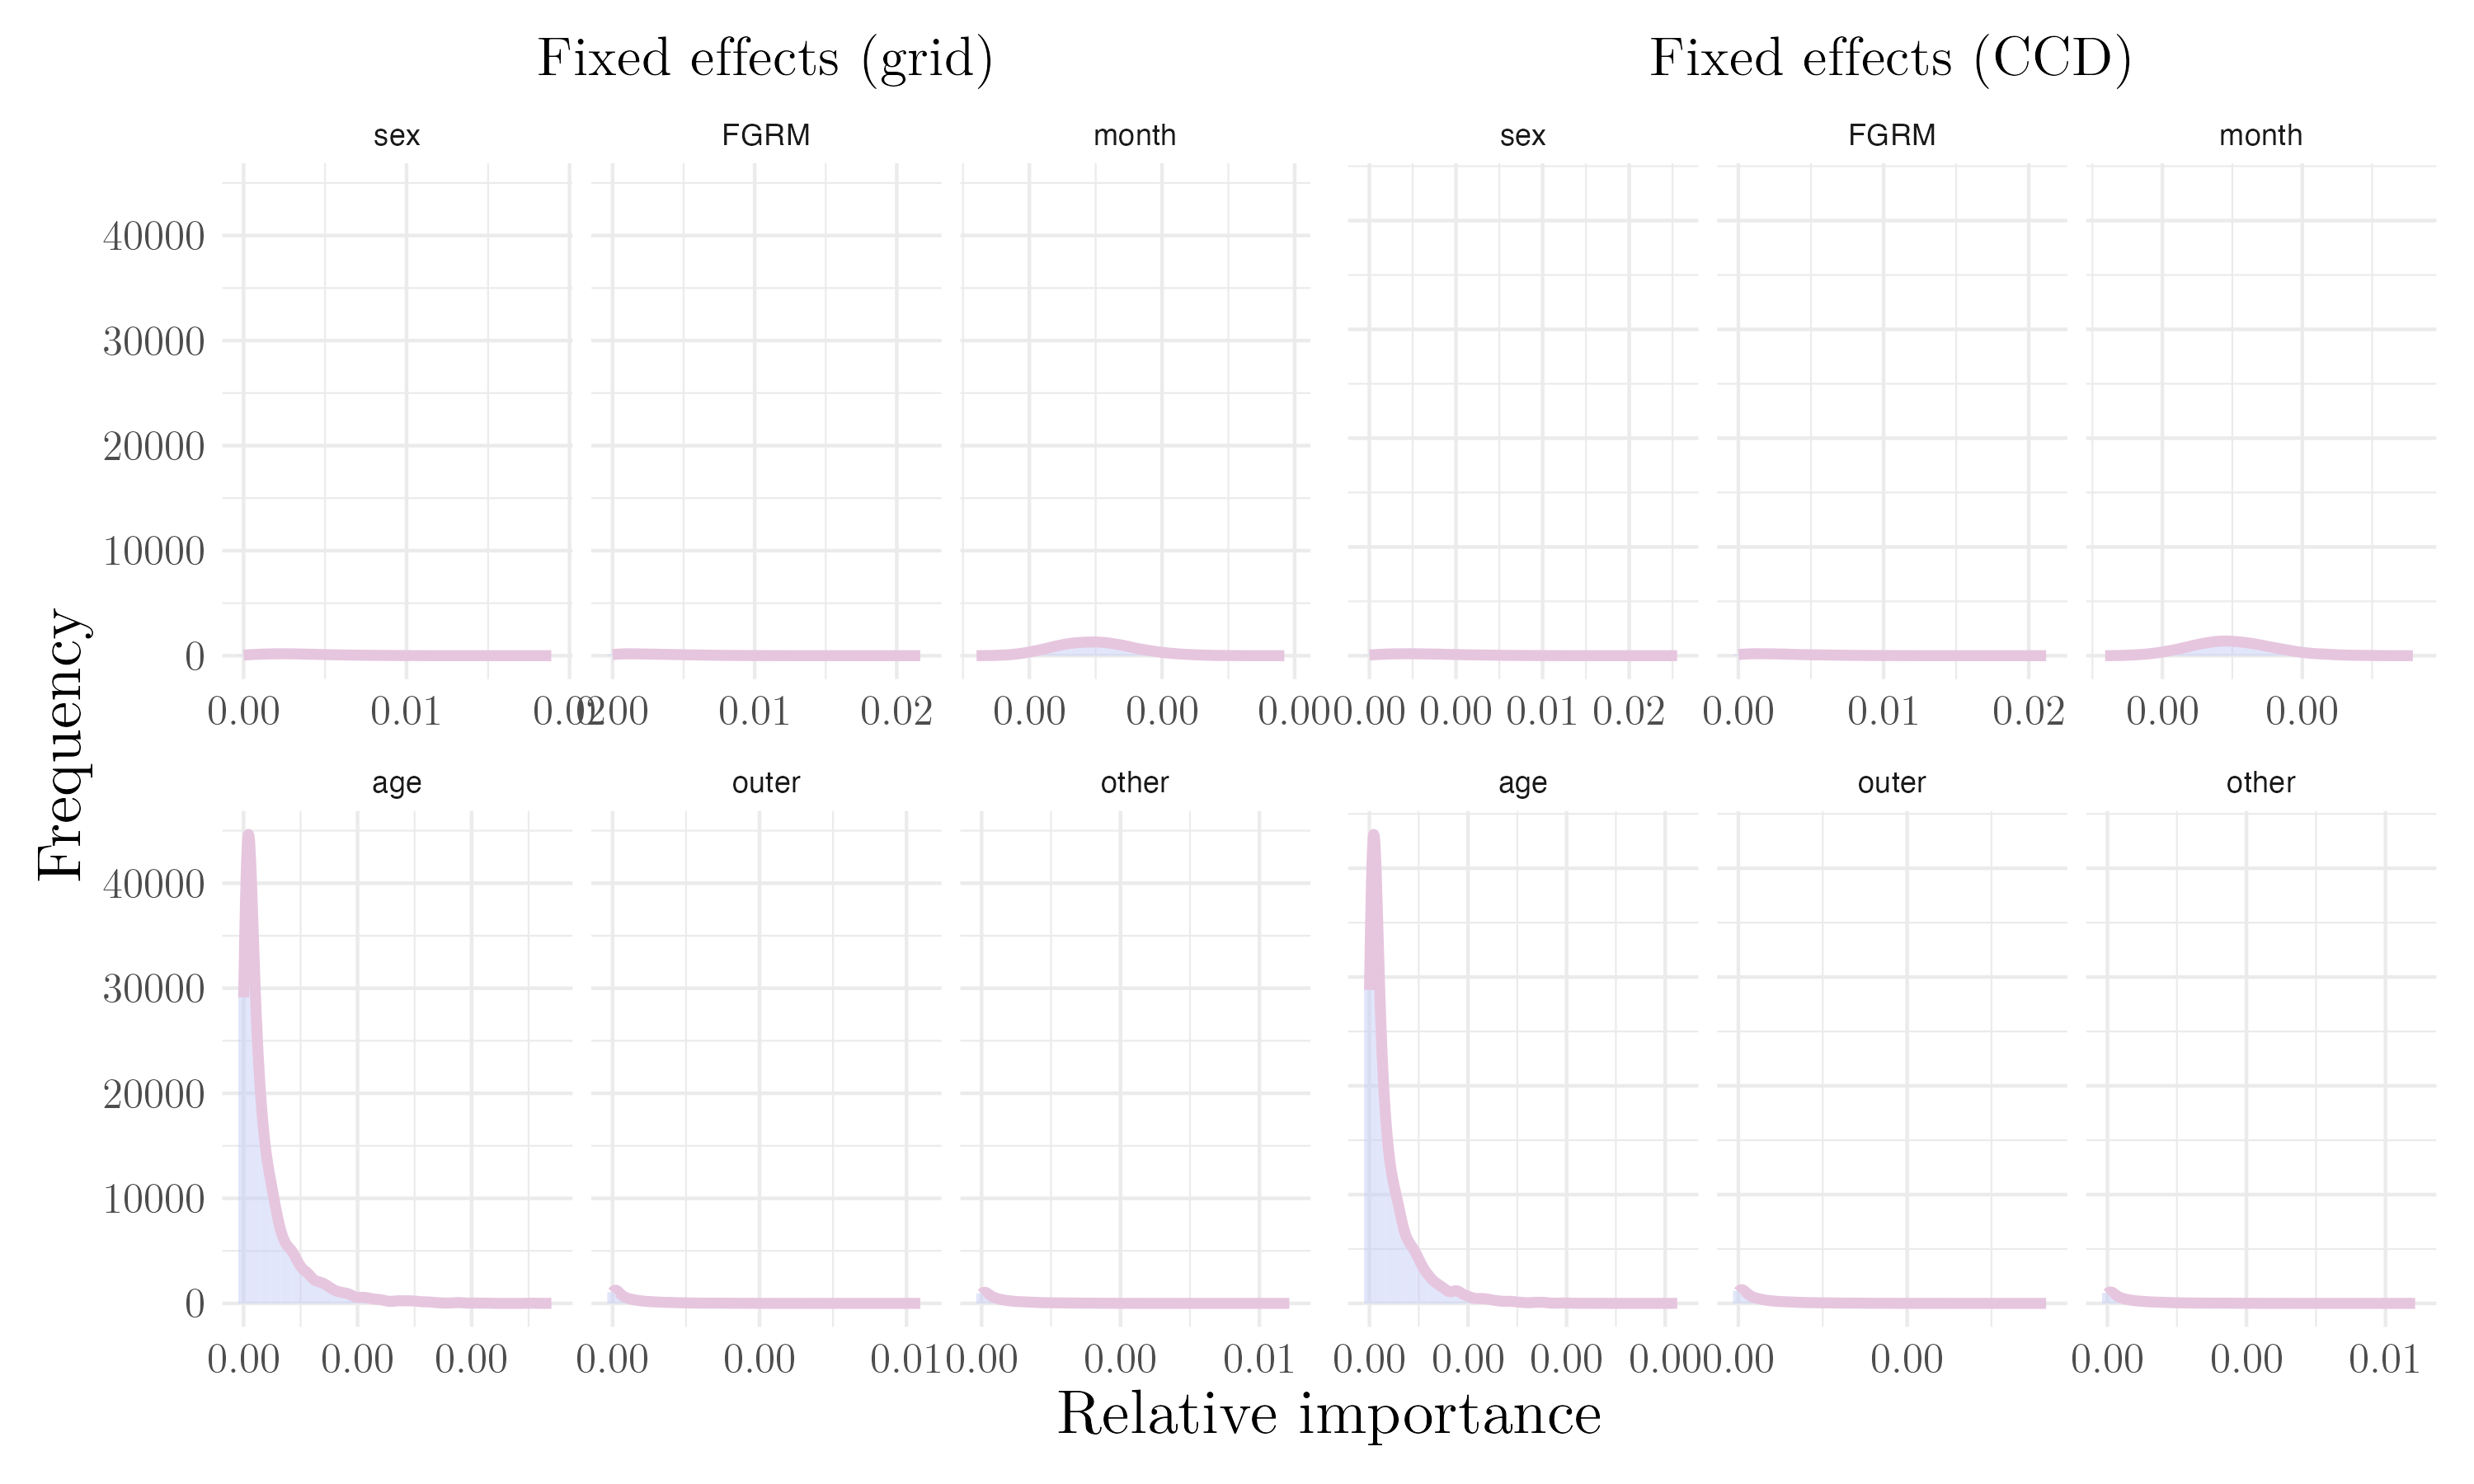
\includegraphics[width=1\linewidth]{Figures/House sparrow study/Tarsus_fixed.png}
%   \caption[Posterior relative importance distributions of all fixed effects in tarsus length model for house sparrow study]{Posterior relative importance distributions of all fixed effects in heritability of tarsus length model for house sparrow study. The grid integration is displayed on the left, and CCD on the right.}
%   \label{fig:tarsus_fixed_sparrows}
% \end{figure}
% In the random effects of the tarsus length model (\Cref{fig:tarsus_random_sparrows}), the Gaussian observations receive the smallest share of importance, while the overdispersive term \textit{IDC} is assigned the largest share. It also seems that the spread of posterior importance distributions for \textit{IDC} and \textit{IDC2} are quite large in this case. As for body mass and wing length, the \textit{hatchyear} covariate is given a small share. The integration strategies agree for the most part, but the grid integration show signs of a trimodal pattern for \textit{IDC} and \textit{IDC2}, with the latter corresponding to the heritability.
% \begin{figure}[H]%\ContinuedFloat
%   \centering
%   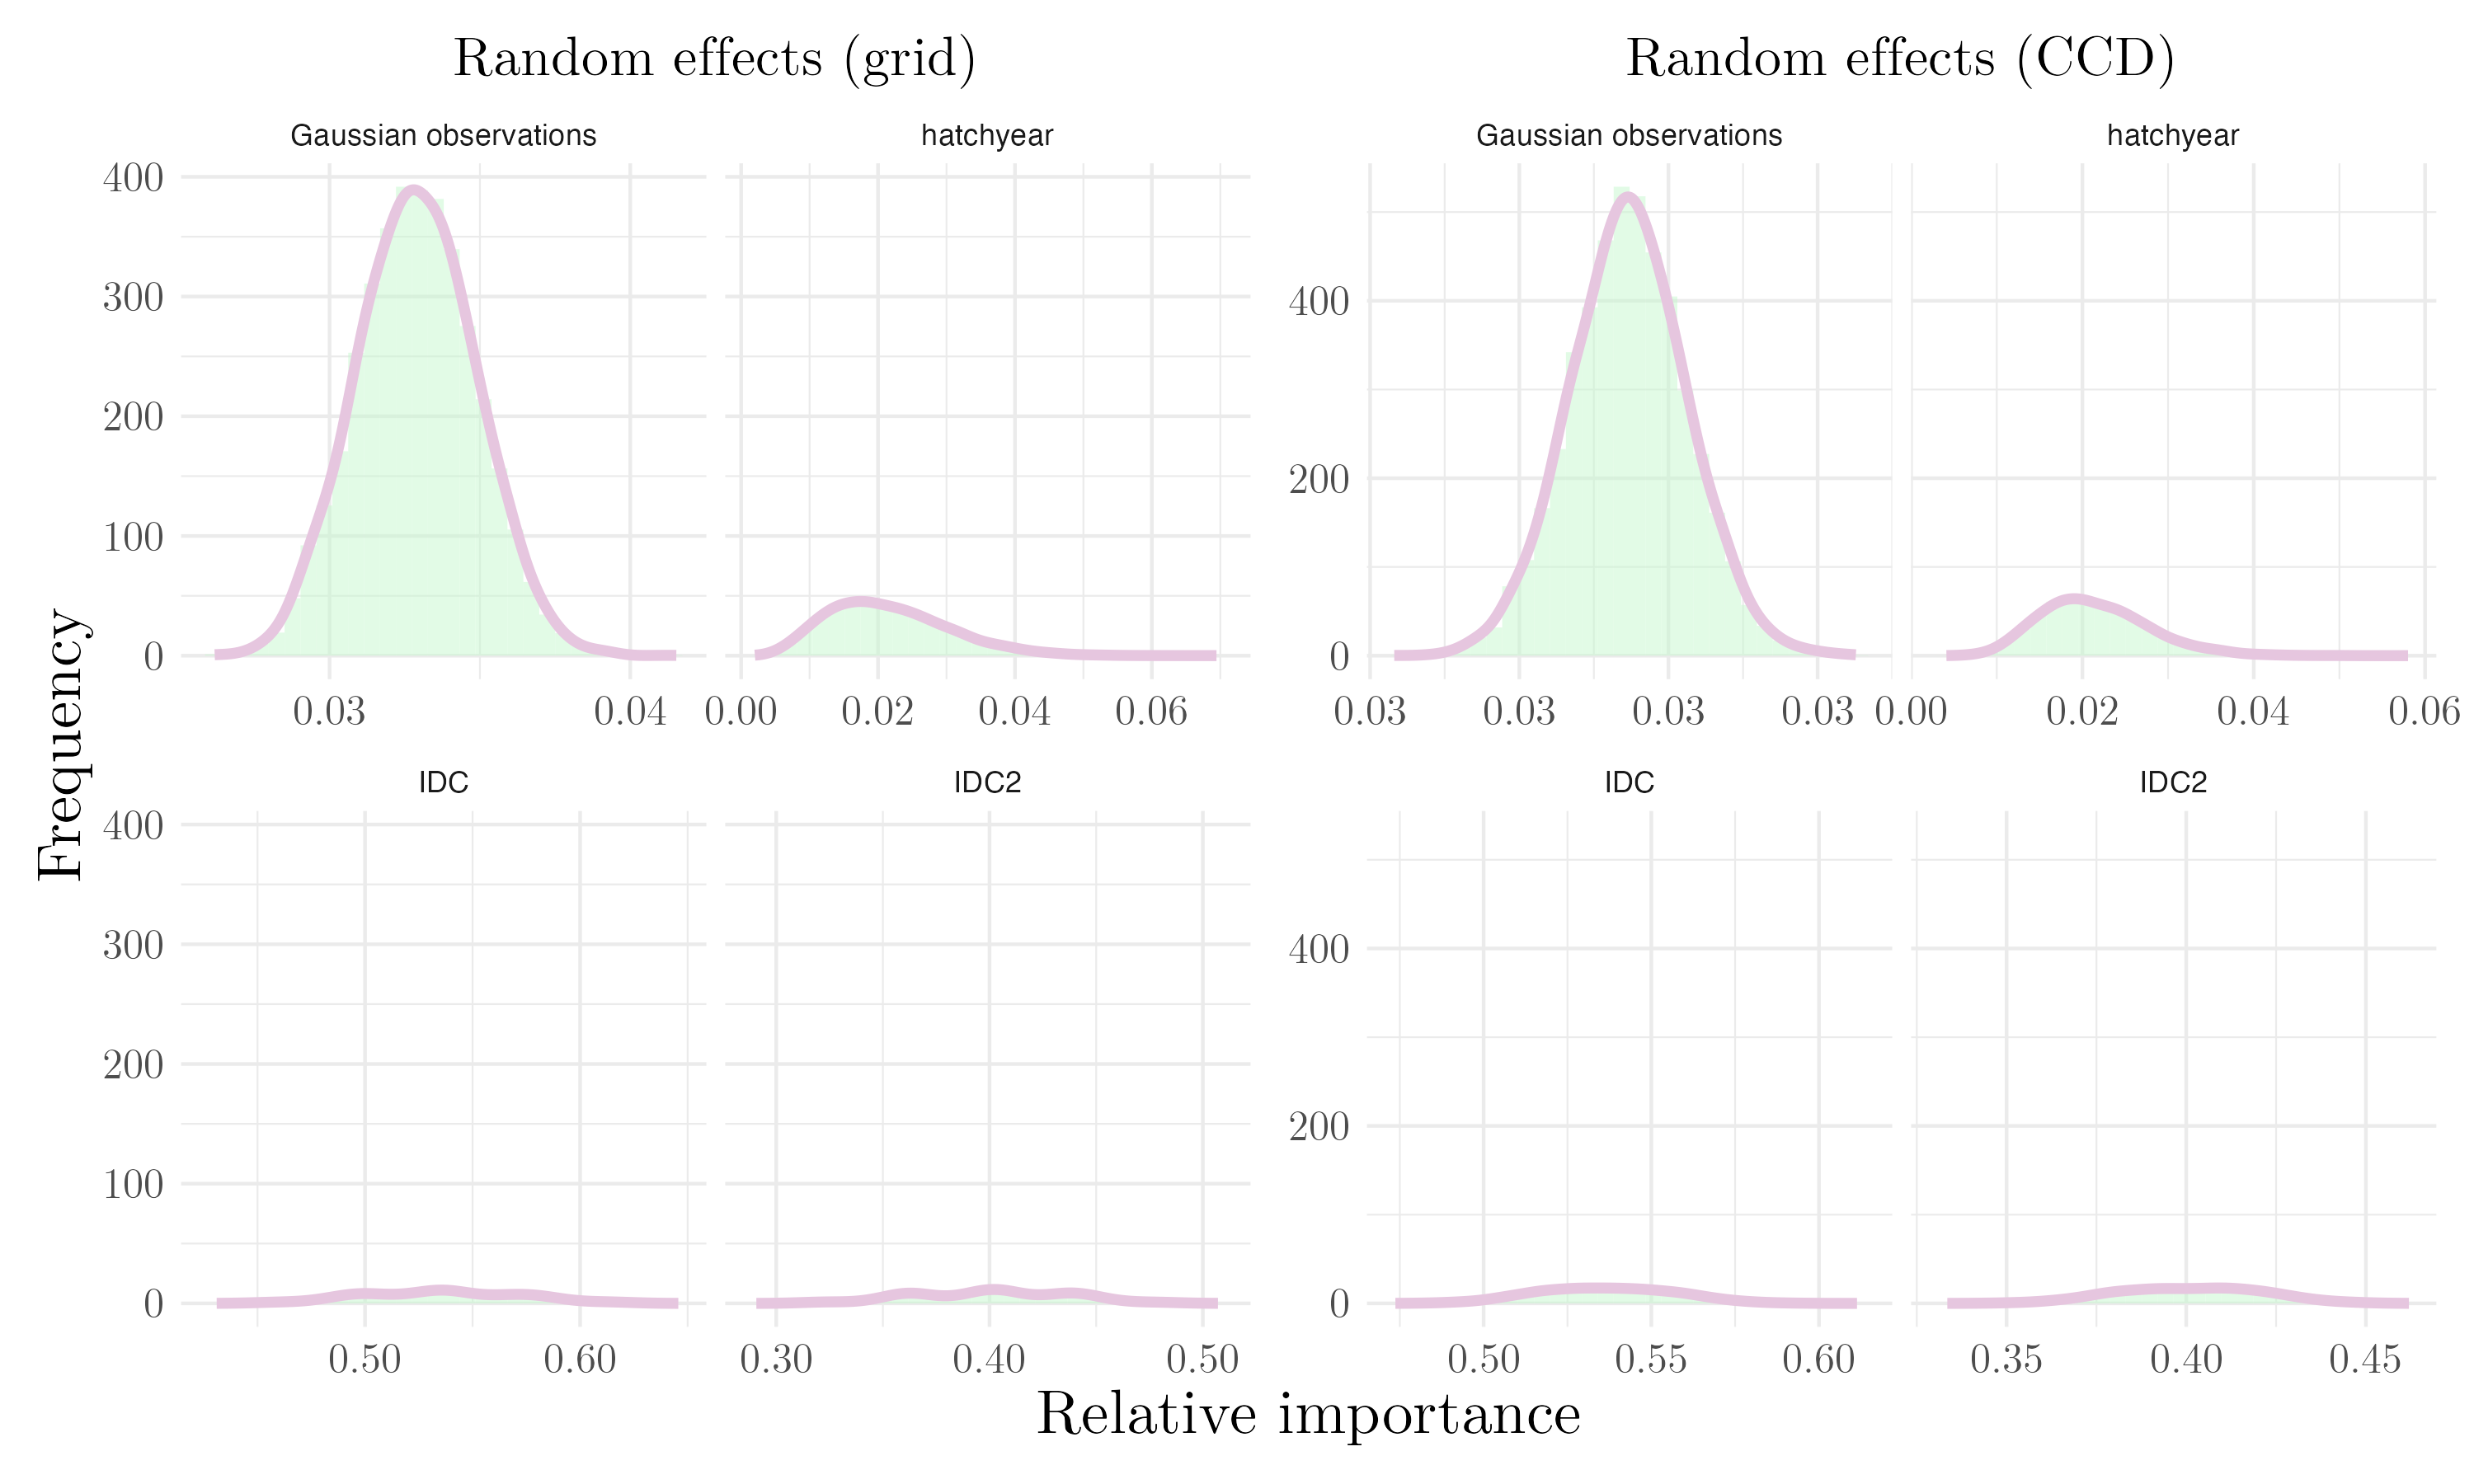
\includegraphics[width=1\linewidth]{Figures/House sparrow study/Tarsus_random.png}
%   \caption[Posterior relative importance distributions of all random effects in tarsus length model for house sparrow study]{Posterior relative importance distributions of all random effects in heritability of tarsus length model for house sparrow study. The grid integration is displayed on the left, and CCD on the right.}
%   \label{fig:tarsus_random_sparrows}
% \end{figure}
% The $R^2$ estimates for the tarsus length model (\Cref{fig:tarsus_r2}) indicate a very small marginal $R^2$, reflecting the minimal importance assigned to the fixed effects. Contrarily, the conditional $R^2$ is extremely high, as the Gaussian observations were given a very small importance. The peaks of the CCD strategy is a bit sharper than that of the grid integration. 
% \begin{figure}[H]%\ContinuedFloat
%   \centering
%   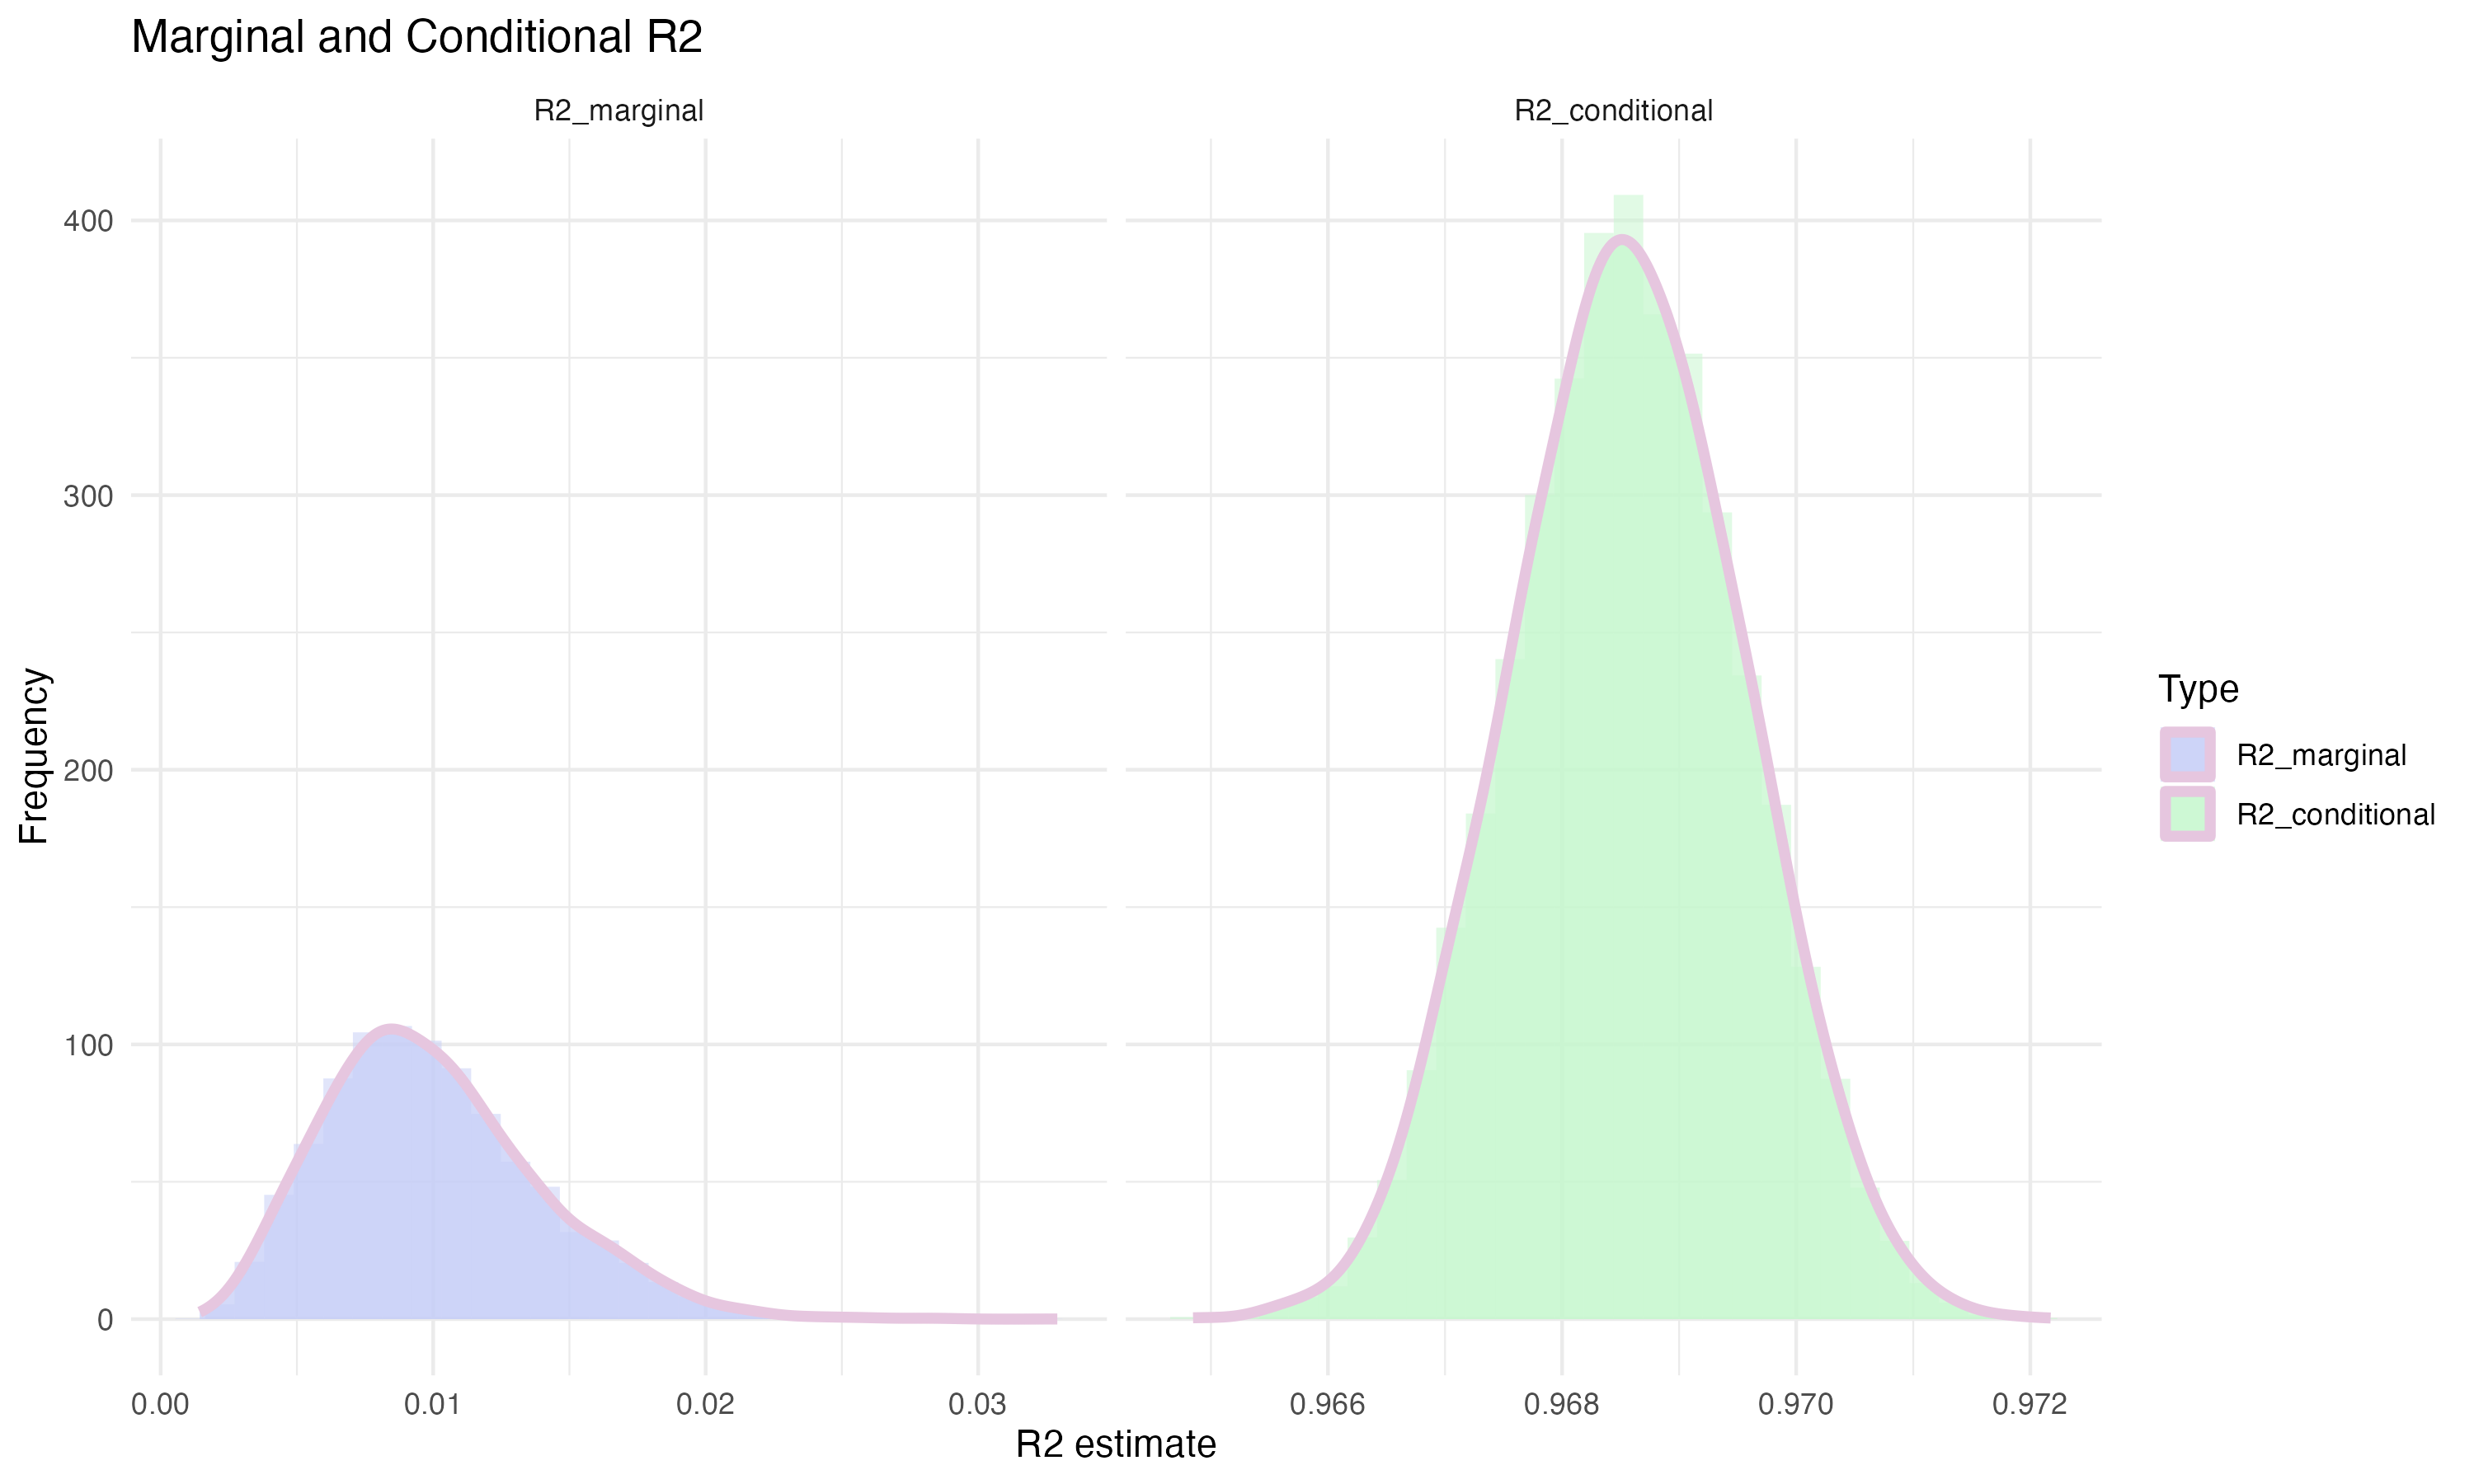
\includegraphics[width=1\linewidth]{Figures/House sparrow study/Tarsus_r2.png}
%   \caption[Posterior distributions of $R^2$ values in tarsus length model for house sparrow study]{Posterior distributions of $R^2$ values in heritability tarsus length model for house sparrow study. The grid integration is displayed on the left, and CCD on the right.}
%   \label{fig:tarsus_r2}
% \end{figure}
\subsection*{Supplementary tables for the non-Gaussian simulation study}
We attach the summarizing tables for the Binomial and Poisson simulation studies here, as they were referred to throughout the thesis. Firstly, \Cref{table:summary_logit} contains summary statistics of the distribution obtained from the Binomial model, while \Cref{table:summary_poisson} contains the same for the Poisson model.
\begin{table}[ht]
    \centering
    \begin{tabular}{@{}llcccccc@{}}
      \toprule
      \multicolumn{2}{c}{\textbf{Measure}} & $\mathbf{\rho=0}$ & $\mathbf{\rho=0.1}$ & $\mathbf{\rho=-0.1}$ & $\mathbf{\rho=0.4}$ & $\mathbf{\rho=-0.4}$ \\ \midrule
      \multirow{3}{*}{\shortstack{Relative Importance of \\ Fixed effect X1}} & Average & 0.098 & 0.118 & 0.077 & 0.173 & 0.020 \\
                                               & 2.5\%   & 0.086 & 0.106 & 0.067 & 0.161 & 0.017 \\
                                               & 97.5\%  & 0.108 & 0.130 & 0.088 & 0.185 & 0.023 \\ \midrule
      \multirow{3}{*}{\shortstack{Relative Importance of \\ Fixed effect X2}} & Average & 0.194 & 0.208 & 0.176 & 0.239 & 0.077 \\
                                               & 2.5\%   & 0.177 & 0.194 & 0.161 & 0.226 & 0.066 \\
                                               & 97.5\%  & 0.210 & 0.223 & 0.193 & 0.251 & 0.087 \\ \midrule
      \multirow{3}{*}{\shortstack{Relative Importance of \\ Fixed effect X3}} & Average & 0.292 & 0.298 & 0.280 & 0.299 & 0.166 \\
                                               & 2.5\%   & 0.272 & 0.280 & 0.258 & 0.285 & 0.150 \\
                                               & 97.5\%  & 0.310 & 0.317 & 0.300 & 0.315 & 0.182 \\ \midrule
      \multirow{3}{*}{\shortstack{Relative Importance of \\ Random effect}} & Average & 0.097 & 0.087 & 0.107 & 0.067 & 0.171 \\
                                               & 2.5\%   & 0.073 & 0.066 & 0.081 & 0.050 & 0.131 \\
                                               & 97.5\%  & 0.121 & 0.117 & 0.139 & 0.086 & 0.211 \\ \midrule
      \multirow{3}{*}{$R^2_m$}            & Average & 0.583 & 0.624 & 0.532 & 0.710 & 0.262 \\
                                           & 2.5\%   & 0.558 & 0.600 & 0.507 & 0.690 & 0.241 \\
                                           & 97.5\%  & 0.607 & 0.646 & 0.557 & 0.730 & 0.284 \\ \midrule
      \multirow{3}{*}{$R^2_c$}            & Average & 0.680 & 0.712 & 0.640 & 0.777 & 0.434 \\
                                           & 2.5\%   & 0.659 & 0.695 & 0.617 & 0.763 & 0.401 \\
                                           & 97.5\%  & 0.700 & 0.731 & 0.660 & 0.792 & 0.468 \\ \bottomrule
    \end{tabular}
    % \begin{tabular}{@{}llcccccc@{}}
    %   \toprule
    %   \multicolumn{2}{c}{\textbf{Measure}} & $\mathbf{\rho=0}$ & $\mathbf{\rho=0.1}$ & $\mathbf{\rho=-0.1}$ & $\mathbf{\rho=0.4}$ & $\mathbf{\rho=-0.4}$ \\ \midrule
    %   \multirow{3}{*}{\shortstack{Relative Importance of \\ Random effect}} & Average & 0.096 & 0.086 & 0.107 & 0.067 & 0.169 \\
    %                                      & 2.5\%   & 0.069 & 0.062 & 0.079 & 0.047 & 0.130 \\
    %                                      & 97.5\%  & 0.126 & 0.112 & 0.139 & 0.089 & 0.219 \\ \midrule
    %   \multirow{3}{*}{\shortstack{Relative Importance of \\ Fixed effect X1}} & Average & 0.097 & 0.117 & 0.077 & 0.173 & 0.020 \\
    %                                        & 2.5\%   & 0.080 & 0.101 & 0.063 & 0.156 & 0.017 \\
    %                                        & 97.5\%  & 0.111 & 0.133 & 0.091 & 0.190 & 0.024 \\ \midrule
    %   \multirow{3}{*}{\shortstack{Relative Importance of \\ Fixed effect X2}} & Average & 0.195 & 0.210 & 0.176 & 0.239 & 0.077 \\
    %                                        & 2.5\%   & 0.174 & 0.188 & 0.156 & 0.222 & 0.064 \\
    %                                        & 97.5\%  & 0.215 & 0.232 & 0.197 & 0.257 & 0.089 \\ \midrule
    %   \multirow{3}{*}{\shortstack{Relative Importance of \\ Fixed effect X3}} & Average & 0.292 & 0.298 & 0.280 & 0.298 & 0.167 \\
    %                                        & 2.5\%   & 0.267 & 0.274 & 0.255 & 0.277 & 0.146 \\
    %                                        & 97.5\%  & 0.318 & 0.321 & 0.307 & 0.318 & 0.187 \\ \midrule
    %   \multirow{3}{*}{$R^2_m$}            & Average & 0.584 & 0.625 & 0.534 & 0.710 & 0.264 \\
    %                                        & 2.5\%   & 0.552 & 0.594 & 0.501 & 0.684 & 0.235 \\
    %                                        & 97.5\%  & 0.614 & 0.654 & 0.565 & 0.732 & 0.290 \\ \midrule
    %   \multirow{3}{*}{$R^2_c$}            & Average & 0.680 & 0.711 & 0.641 & 0.778 & 0.433 \\
    %                                        & 2.5\%   & 0.653 & 0.684 & 0.613 & 0.758 & 0.392 \\
    %                                        & 97.5\%  & 0.705 & 0.735 & 0.668 & 0.797 & 0.477 \\ \bottomrule
    % \end{tabular}
    \caption[Summary statistics for binomial GLMM simulation study]{Summary of simulation study results for the quantiles of relative importance estimates of the Logit model across different correlation levels. For $\rho=0$ the expected values are given in \Cref{table:3}.}
    \label{table:summary_logit}
\end{table}
\begin{table}[ht]
    \centering
    \begin{tabular}{@{}llcccccc@{}}
      \toprule
      \multicolumn{2}{c}{\textbf{Measure}} & $\mathbf{\rho=0}$ & $\mathbf{\rho=0.1}$ & $\mathbf{\rho=-0.1}$ & $\mathbf{\rho=0.4}$ & $\mathbf{\rho=-0.4}$ \\ \midrule
      \multirow{3}{*}{\shortstack{Relative Importance of \\ Fixed effect X1}} & Average & 0.097 & 0.119 & 0.075 & 0.181 & 0.017 \\
                                           & 2.5\%   & 0.088 & 0.109 & 0.066 & 0.172 & 0.015 \\
                                           & 97.5\%  & 0.107 & 0.128 & 0.084 & 0.189 & 0.020 \\ \midrule
      \multirow{3}{*}{\shortstack{Relative Importance of \\ Fixed effect X2}} & Average & 0.193 & 0.212 & 0.171 & 0.251 & 0.066 \\
                                           & 2.5\%   & 0.181 & 0.200 & 0.158 & 0.241 & 0.057 \\
                                           & 97.5\%  & 0.205 & 0.224 & 0.184 & 0.260 & 0.075 \\ \midrule
      \multirow{3}{*}{\shortstack{Relative Importance of \\ Fixed effect X3}} & Average & 0.290 & 0.302 & 0.272 & 0.314 & 0.143 \\
                                           & 2.5\%   & 0.276 & 0.288 & 0.256 & 0.302 & 0.130 \\
                                           & 97.5\%  & 0.307 & 0.316 & 0.289 & 0.326 & 0.156 \\ \midrule
      \multirow{3}{*}{\shortstack{Relative Importance of \\ Random effect}} & Average & 0.098 & 0.090 & 0.106 & 0.072 & 0.149 \\
                                           & 2.5\%   & 0.074 & 0.068 & 0.081 & 0.054 & 0.111 \\
                                           & 97.5\%  & 0.127 & 0.112 & 0.136 & 0.093 & 0.190 \\ \midrule
      \multirow{3}{*}{$R^2_m$}            & Average & 0.580 & 0.633 & 0.519 & 0.746 & 0.225 \\
                                           & 2.5\%   & 0.558 & 0.613 & 0.496 & 0.727 & 0.207 \\
                                           & 97.5\%  & 0.601 & 0.654 & 0.541 & 0.763 & 0.244 \\ \midrule
      \multirow{3}{*}{$R^2_c$}            & Average & 0.679 & 0.723 & 0.625 & 0.817 & 0.374 \\
                                           & 2.5\%   & 0.658 & 0.704 & 0.602 & 0.804 & 0.337 \\
                                           & 97.5\%  & 0.700 & 0.741 & 0.648 & 0.830 & 0.413 \\ \bottomrule
    \end{tabular}
    % \begin{tabular}{@{}llcccccc@{}}
    %   \toprule
    %   \multicolumn{2}{c}{\textbf{Measure}} & $\mathbf{\rho=0}$ & $\mathbf{\rho=0.1}$ & $\mathbf{\rho=-0.1}$ & $\mathbf{\rho=0.4}$ & $\mathbf{\rho=-0.4}$ \\ \midrule
    %   \multirow{3}{*}{\shortstack{Relative Importance of \\ Random effect}} & Average & 0.095 & 0.088 & 0.104 & 0.072 & 0.147 \\
    %                                      & 2.5\%   & 0.070 & 0.066 & 0.073 & 0.053 & 0.107 \\
    %                                      & 97.5\%  & 0.124 & 0.117 & 0.137 & 0.093 & 0.194 \\ \midrule
    %   \multirow{3}{*}{\shortstack{Relative Importance of \\ Fixed effect X1}} & Average & 0.097 & 0.119 & 0.075 & 0.181 & 0.017 \\
    %                                        & 2.5\%   & 0.085 & 0.106 & 0.064 & 0.171 & 0.014 \\
    %                                        & 97.5\%  & 0.108 & 0.131 & 0.086 & 0.192 & 0.021 \\ \midrule
    %   \multirow{3}{*}{\shortstack{Relative Importance of \\ Fixed effect X2}} & Average & 0.194 & 0.213 & 0.171 & 0.251 & 0.066 \\
    %                                        & 2.5\%   & 0.180 & 0.199 & 0.155 & 0.240 & 0.054 \\
    %                                        & 97.5\%  & 0.210 & 0.229 & 0.187 & 0.263 & 0.079 \\ \midrule
    %   \multirow{3}{*}{\shortstack{Relative Importance of \\ Fixed effect X3}} & Average & 0.292 & 0.303 & 0.273 & 0.313 & 0.142 \\
    %                                        & 2.5\%   & 0.2725 & 0.2848 & 0.2522 & 0.2994 & 0.124 \\
    %                                        & 97.5\%  & 0.3102 & 0.3213 & 0.2925 & 0.3258 & 0.162 \\ \midrule
    %   \multirow{3}{*}{$R^2_m$}            & Average & 0.5827 & 0.6343 & 0.519 & 0.746 & 0.225 \\
    %                                        & 2.5\%   & 0.557 & 0.610 & 0.494 & 0.726 & 0.201 \\
    %                                        & 97.5\%  & 0.606 & 0.657 & 0.541 & 0.765 & 0.250 \\ \midrule
    %   \multirow{3}{*}{$R^2_c$}            & Average & 0.678 & 0.723 & 0.623 & 0.818 & 0.371 \\
    %                                        & 2.5\%   & 0.656 & 0.702 & 0.595 & 0.803 & 0.335 \\
    %                                        & 97.5\%  & 0.700 & 0.743 & 0.648 & 0.832 & 0.414 \\ \bottomrule
    % \end{tabular}
    \caption[Summary statistics for Poisson GLMM simulation study]{Summary of simulation study results for the quantiles of relative importance estimates the Poisson model across different correlation levels. For $\rho=0$ the expected values are given in \Cref{table:3}.}
    \label{table:summary_poisson}
  \end{table}